\documentclass[10pt,reqno]{book}
\usepackage{amsmath,amssymb,amsfonts,amsthm}
\usepackage{tikz,caption}
\usepackage{emptypage}
\usepackage{pgfplots}
\usepackage{algorithm}
\usepackage[noend]{algpseudocode}
\usepackage{listings}
\usepackage{booktabs}
\usepackage{graphicx}
\graphicspath{ {images1/} }
\usepackage{ mathrsfs }
\usepackage{bm}
\usepackage{tikz-3dplot}
\usetikzlibrary{patterns}
\usetikzlibrary{3d}
\usetikzlibrary{decorations.pathmorphing,patterns,angles}
\usetikzlibrary{decorations.pathreplacing,decorations.markings}
\pgfplotsset{compat=1.8}
\usepackage{subcaption,array}
\usepackage{tikz-qtree}
\usepackage{mathtools}
\newcommand{\verteq}{\rotatebox{90}{$\,=$}}
\newcommand{\equalto}[2]{\underset{\scriptstyle\overset{\mkern4mu\verteq}{#2}}{#1}}

\usepgfplotslibrary{fillbetween}
\usetikzlibrary{patterns}

% Tikz stuff
\tikzset{
	% style to apply some styles to each segment of a path
	on each segment/.style={
		decorate,
		decoration={
			show path construction,
			moveto code={},
			lineto code={
				\path [#1]
				(\tikzinputsegmentfirst) -- (\tikzinputsegmentlast);
			},
			curveto code={
				\path [#1] (\tikzinputsegmentfirst)
				.. controls
				(\tikzinputsegmentsupporta) and (\tikzinputsegmentsupportb)
				..
				(\tikzinputsegmentlast);
			},
			closepath code={
				\path [#1]
				(\tikzinputsegmentfirst) -- (\tikzinputsegmentlast);
			},
		},
	},
	% style to add an arrow in the middle of a path
	mid arrow/.style={postaction={decorate,decoration={
				markings,
				mark=at position .5 with {\arrow[#1]{stealth}}
	}}},
}


\DeclareGraphicsExtensions{.pdf}
\parindent 1cm
\parskip 0.2cm
\topmargin 0.2cm
\oddsidemargin 1cm
\evensidemargin 0.5cm
\textwidth 15cm
\textheight 21cm
\theoremstyle{definition}
\newtheorem{theorem}{Theorem}[section]
\newtheorem{proposition}[theorem]{Proposition}
\newtheorem{corollary}[theorem]{Corollary}
\newtheorem{lemma}[theorem]{Lemma}
\newtheorem{remark}[theorem]{Remark}
\newtheorem{definition}[theorem]{Definition}
\newtheorem{example}{Example}
\renewcommand{\qedsymbol}{$\blacksquare$}

\renewcommand{\vec}[1]{\mathbf{#1}}


\newcommand{\uvec}[1]{\boldsymbol{\hat{\textbf{#1}}}}

\def\L{\mathscr{L}}
\def\R{\mathbb{R}}
\def\S{\mathbb{S}}
\def\I{\mathbb{I}}
\makeindex

% sqare of half axes
\newcommand{\asa}{2}
\newcommand{\bsa}{0.5}
\newcommand{\csa}{0.5}

\font\myfont=cmr12 at 20pt

\title{\myfont{Calculus III}}

\author{Lukas Zamora}

\date{November 28, 2017}
\pagestyle{headings}
\pagenumbering{roman}



\begin{document}

	\maketitle
	\addcontentsline{toc}{chapter}{Contents}
	\pagenumbering{arabic}

	\tableofcontents

	\chapter{Vectors}

	\section{The Basics}

	Vectors are used to represent quantities that have both a magnitude and a direction.  Good examples of quantities that can be represented by vectors are force and velocity.  Both of these have a direction and a magnitude. Consider the sketch below
	\begin{center}
		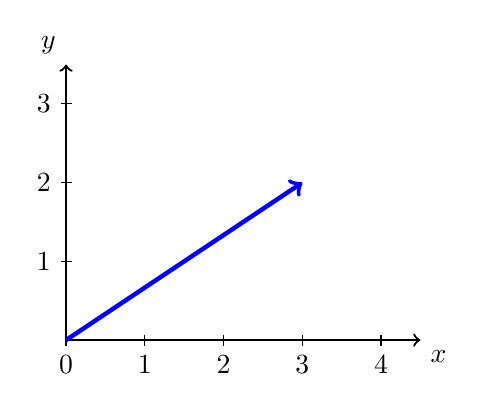
\begin{tikzpicture}
			\draw[thick,->] (0,0) -- (4.5,0) node[anchor=north west] {$x$};
			\draw[thick,->] (0,0) -- (0,3.5) node[anchor=south east] {$y$};
  			 \foreach \x in {0,1,2,3,4}
   			 	\draw (\x cm,2pt) -- (\x cm,-2pt) node[anchor=north] {$\x$};
			\foreach \y in {1,2,3}
				\draw (2pt,\y cm) -- (-2pt,\y cm) node[anchor=east] {$\y$};
			\draw[ultra thick,draw=blue,->] (0,0) -- (3,2);
  		\end{tikzpicture}
	\end{center}
	In this case the vector starts at a specific point then moves 3 units to the right and 2 units up. The notation that we'll use for this vector is,
	\[ \vec{v} = \langle 3,2 \rangle \]
	and each of the directed line segments in the sketch are called \textit{representations} of the vector. Be careful to distinguish vector notation, $ \langle 3,2 \rangle $, from the notation we use to represent coordinates of points, $(3,2)$. The vector denotes a magnitude and a direction of a quantity while the point denotes a location in space. So don't mix the notations up!\\ \\
	A representation of the vector $ \vec{v} = \langle a_1,a_2 \rangle $ in two dimensional space is any directed line segment, $\overrightarrow{AB}$, from the point $A=(x,y)$ to the point $B = (x+a_1, y+a_2)$. Likewise a representation of the vector $\vec{v} = \langle a_1,a_2,a_3 \rangle$ in three dimensional space is any directed line segment, $\overrightarrow{AB}$, from the point $A=(x,y,z)$ to the point $B = (x+a_1,y+a_2,z+a_3)$. Note that there is very little difference between the two dimensional and three dimensional formulas. To get from the three dimensional formula to the two dimensional formula all we did is take out the third component/coordinate. Because of this most of the formulas here are given only in their three dimensional version. If we need them in their two dimensional form we can easily modify the three dimensional form.\\ \\
	The representation of the vector $\vec{v} = \langle a_1,a_2,a_3 \rangle$ that starts at the point $A=(0,0,0)$ and ends at the point $B=(a_1,a_2,a_3)$ is called the \textit{position vector} of the point $(a_1,a_2,a_3)$. Position vecotrs are useful if we ever need to represent a point as a vector.\\ \\
	The \textit{magnitude}, or length of the vector $\vec{v} = \langle a_1,a_2,a_3 \rangle$ is given by,
	\[ || \vec{v} || = \sqrt{a_1^2 + a_2^2 + a_3^2} \]
	We also have the fact that
	\[ \text{If } ||\vec{a}|| = 0 \text{ then } \vec{a} = \vec{0} \]
	Which makes sense. Because we square all the components the only way we can get zero out of the formula was for the components to be zero in the first place.\\ \\
	Any vector with magnitude of 1, is called the \textit{unit vector}. Given a vector $\vec{v}$, $\vec{u} = \displaystyle{\frac{\vec{v}}{||\vec{v}||}}$ will be a unit vector that points in the same direction as $\vec{v}$. The vector whose components are all zeros, is called the \textit{zero vector}, denoted by $\vec{0}$.\\ \\
	In $\R^3$, there are unit vectors that are called the \textit{standard basis vectors}. They are denoted by 
	\[ \uvec{\i} = \langle 1,0,0 \rangle \qquad \uvec{\j} = \langle 0,1,0 \rangle \qquad \uvec{k} = \langle 0,0,1 \rangle \]
	which are also unit vectors.

	\section{Vector Arithmetic}

	Given the vectors $\vec{a} = \langle a_1,a_2,a_3 \rangle$ and $\vec{b} = \langle b_1,b_2,b_3 \rangle$, the addition of  the two vectors is given by
	\[ \vec{a} + \vec{b} = \langle a_1+b_1,a_2+b_2,a_3+b_3 \rangle \]
	The following figure gives the geometric interpretation of the addition of two vectors
	\begin{center}
		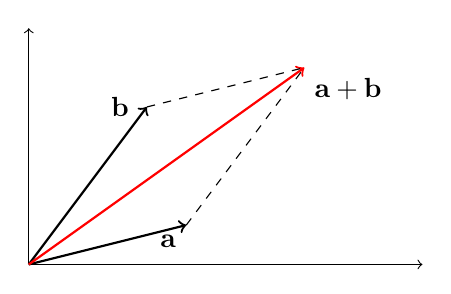
\begin{tikzpicture}
			\draw[->] (0,0) -- (0,3);
			\draw[->] (0,0) -- (5,0);
			\draw[thick, ->] (0,0) -- (1.5,2)node[left=1mm] {$\vec{b}$};
			\draw[thick,->] (0,0) -- (2,0.5) node[below left] {$\vec{a}$};
			\draw[thick, draw=red,->] (0,0) -- (3.5,2.5) node[below right] {$\vec{a} + \vec{b}$};
			\draw[dashed] (2,0.5) -- (3.5,2.5);
			\draw[dashed] (1.5,2) -- (3.5,2.5);
		\end{tikzpicture}
	\end{center}
	Substraction is very similar. Given the vectors $\vec{a} = \langle a_1,a_2,a_3 \rangle$ and $\vec{b} = \langle b_1,b_2,b_3 \rangle$, the difference of the two vectors is given by
	\[ \vec{a} - \vec{b} = \langle a_1-b_1,a_2-b_2,a_3-b_3 \rangle \]
	Here is the geometric interpretation of the difference of two vectors
	\begin{center}
		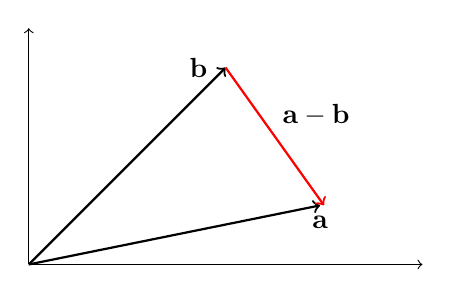
\begin{tikzpicture}
			\draw[->] (0,0) -- (0,3);
			\draw[->] (0,0) -- (5,0);
			\draw[thick,->] (0,0) -- (2.5,2.5) node[left=1mm] {$\vec{b}$};
			\draw[thick,->] (0,0) -- (3.7,0.75) node[below] {$\vec{a}$};
			\draw[thick, ->,draw=red] (2.5,2.5) -- (3.75,0.75);
			\draw (3.1,1.9) node[right] {$\vec{a} - \vec{b}$};
		\end{tikzpicture}
	\end{center}
	The next arithmetic operation that we want to look at is \textit{scalar multiplication}. Given the vector $\vec{a} = \langle a_1,a_2,a_3 \rangle$ and any number $r$ the scalar multiplication is 
	\[ r\vec{a} = \langle ra_1,ra_2,ra_3 \rangle \]
	Here is its geometric interpretation. Suppose $r=2$, then
	\begin{center}
		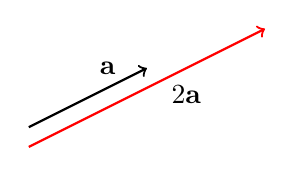
\begin{tikzpicture}
			\draw[thick, draw=red,->] (0,0) -- (3,1.5);
			\draw[thick,->] (0,0.25) -- (1.5,1);
			\draw (1,1) node {$\vec{a}$};
			\draw (2,1) node[below=1mm] {$2\vec{a}$};
		\end{tikzpicture}
	\end{center}
	Two vectors are parallel if they have the same direction or are in exactly opposite directions. Let's suppose that $\vec{a}$ and $\vec{b}$ are parallel vectors. If they are parallel then there must be a number $r$ so that, 
	\[ \vec{a} = r\vec{b} \]
	So, two vectors are parallel if one is a scalar multiple of the other.\\ \\
	In the previous section we introduced the idea of standard basis vectors without discussing why they were important, so let's do that. Start with the vector
	\[ \vec{a} = \langle a_1,a_2,a_3 \rangle \]
	We can use the addition of vectors to break this up
	\begin{align*}
		\vec{a} &= \langle a_1,a_2,a_3 \rangle\\
				&= \langle a_1,0,0 \rangle + \langle 0,a_2,0 \rangle + \langle 0,0,a_3 \rangle
	\end{align*}
	and use scalar multiplication to break this up as follows
	\begin{align*}
		\vec{a} &= \langle a_1,0,0 \rangle + \langle 0,a_2,0 \rangle + \langle 0,0,a_3 \rangle \\
				&= a_1 \langle 1,0,0 \rangle + a_2 \langle 0,1,0 \rangle + \langle 0,0,1 \rangle
	\end{align*}
	Notice how these are just the three standard basis vectors for $\R^3$
	\[ \vec{a} = a_1\uvec{\i} + a_2\uvec{\j} + a_3\uvec{k} \]
	So we can take any vector and write it in terms of the standard basis vectors.\\ \\
	\textbf{Properties}\\
	If $\vec{u}$, $\vec{v}$, and $\vec{w}$ are vectors (each with the same number of components) and $a$ and $b$ are two numbers, then we have the following properties

	\begin{center}
		\begin{tabular}{lcl}
			$\vec{u} + \vec{v} = \vec{v} + \vec{u}$ & & $\vec{u} + (\vec{v} + \vec{w}) = 	(\vec{u} + \vec{v}) + \vec{w}$\\	
			$\vec{u} + 0 = \vec{u}$ & & $1 \cdot \vec{u} = \vec{u}$\\	
			$a(\vec{u} + \vec{v}) = a\vec{u} + a\vec{v}$ & & $(a+b)\vec{u} = a\vec{u} + b	\vec{u}$
		\end{tabular}
	\end{center}

	\section{Dot Product}

	Given two vectors $\vec{a} = \langle a_1,a_2,a_3 \rangle$ and $\vec{b} = \langle b_1,b_2,b_3 \rangle$ the dot product is,
	\begin{equation}
		\vec{a} \cdot \vec{b} = a_1b_1 + a_2b_2 + a_3b_3
	\end{equation}
	Notice how our answer is just a scalar, not a vector. Here are some properties of the dot product.\\ \\
	\textbf{Properties}\\
	If $\vec{u}$, $\vec{v}$, and $\vec{w}$ are vectors and $c$ is a number then,
	\begin{center}
		\begin{tabular}{lcl}
			$\vec{u} \cdot (\vec{v} + \vec{w}) = \vec{u} \cdot \vec{v} + \vec{u} \cdot \vec{w}$ & & $(c\vec{u}) \cdot \vec{v} = \vec{u} \cdot (c\vec{v}) = c (\vec{u} \cdot \vec{v})$\\
			$\vec{u} \cdot \vec{v} = \vec{v} \cdot \vec{u}$ & & $\vec{u} \cdot \vec{0} = 0$\\
			$\vec{u} \cdot \vec{u} = ||\vec{u}||^2$ & & If $\vec{u} \cdot \vec{u} = 0$ then $\vec{u} = \vec{0}$
		\end{tabular}
	\end{center}
	There is also a nice geometric interpretation to the dot product. First suppose that $\theta$ is the angle between $\vec{a}$ and $\vec{b}$ such that $0 \leq \theta \leq \pi$ as shown in the figure below.

	\begin{center}
		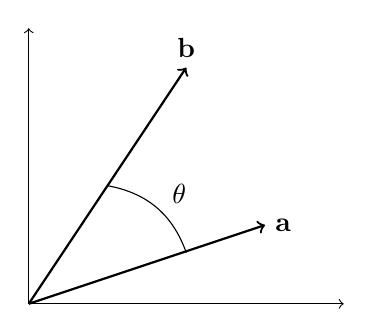
\begin{tikzpicture}
			\draw[->] (0,0) -- (0,3.5);
			\draw[->] (0,0) -- (4,0); 
			\draw[thick, ->] (0,0) -- (2,3) node[above] {$\vec{b}$};
			\draw[thick, ->] (0,0) -- (3,1) node[right] {$\vec{a}$};
			\draw (1,1.5) to [bend left] (2,0.65);
			\draw (1.7,1.4) node[right] {$\theta$};
		\end{tikzpicture}
	\end{center}
	We can then have the following theorem\\ \\
	\begin{theorem}
		\[\vec{a} \cdot \vec{b} = ||\vec{a}|| \, ||\vec{b}||\cos(\theta)\]
	\end{theorem}
	\noindent The formula from this theorem is often used not to compute a dot product but instead to find the angle between two vectors.\\ \\
	The dot product gives us a very nice method for determining if two vectors are perpendicular and it will give another method for determining when two vectors are parallel.  Note as well that often we will use the term \textit{orthogonal} in place of perpendicular. If two vectors are orthogonal then we know that the angle between them is 90 degrees. From (1.3.1) this tells us that if two vectors are orthogonal then,
	\[ \vec{a} \cdot \vec{b} = 0 \]
	Likewise, if two vectors are parallel then the angle between them is either 0 degrees (pointing in the same direction) or 180 degrees (pointing in the opposite direction). Once again using (1.3.1) this would mean that one of the following would have to be true
	\[ \vec{a} \cdot \vec{b} = ||\vec{a}|| \, ||\vec{b}|| (\theta = 0^o) \qquad \text{or} \qquad \vec{a} \cdot \vec{b} = -||\vec{a}|| \, ||\vec{b}|| (\theta = 180^o) \]

	\subsubsection*{Projections}

	Given two vectors $\vec{a}$ and $\vec{b}$ we want to determine the projection of $\vec{b}$ onto $\vec{a}$. The projection is denoted by $ \text{proj}_{\vec{a}}\vec{b}$. Here are a couple of sketches illustrating the projection
	\begin{center}
		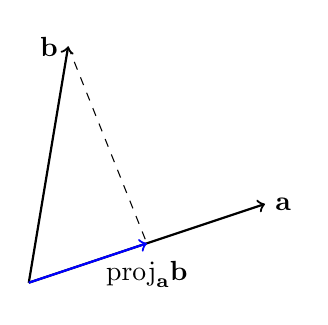
\begin{tikzpicture}
			\draw[thick,->] (0,0) -- (3,1) node[right] {$\vec{a}$};
			\draw[thick,->] (0,0) -- (0.5,3) node[left] {$\vec{b}$};
			\draw[thick, ->,draw=blue] (0,0) -- (1.5,0.5) node [below=1mm] {$\text{proj}_	{\vec{a}}\vec{b}$};	
			\draw[dashed] (0.5,	3) -- (1.5,0.5);	
		\end{tikzpicture}\hspace{1cm}	
		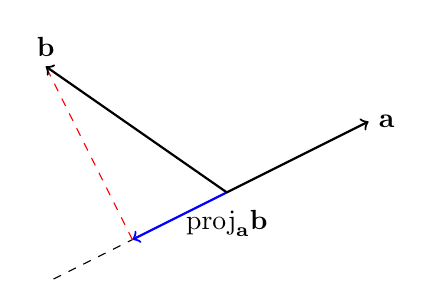
\begin{tikzpicture}	
			\draw[dashed] (	0,0) -- (1,0.5);	
			\draw[thick, <-	,draw=blue] (1,0.5) -- (2.2,1.1) node[below=1mm] {$\text{proj}	_{\vec{a}}\vec{	b}$};	
			\draw[thick, ->	] (2.	2,1.1) -- (4,2) node[right] {$\vec{a}$};	
			\draw[dashed,draw=red] (1,0.5) -- (-.1,2.7);	
			\draw[thick,->] (2.2,1.1) -- (-0.1,2.7) node[above] {$\vec{b}$};
		\end{tikzpicture}
	\end{center}
	So, to get the projection of $\vec{b}$ onto $\vec{a}$ we drop straight down from the end of $\vec{b}$ until we hit (and form a right angle) with the line that is parallel to $\vec{a}$. The projection is then the vector that is parallel to $\vec{a}$, starts at the same point both of the original vectors started at and ends where the dashed line hits the line parallel to $\vec{a}$. Here is a nice formula for finding the projection of $\vec{b}$ onto $\vec{a}$,
	\[ \text{proj}_{\vec{a}}\vec{b} = \frac{\vec{a} \cdot \vec{b}}{||\vec{a}||^2}\vec{a} \]
	Note that we also need to be very careful with notation here. The projection of $\vec{a}$ onto $\vec{b}$ is given by
	\[ \text{proj}_{\vec{b}}\vec{a} = \frac{\vec{a} \cdot \vec{b}}{||\vec{b}||^2}\vec{b} \]

	\section{Cross Product}

	Given two vectors $\vec{a} = \langle a_1,a_2,a_3 \rangle$ and $\vec{b} = \langle b_1, b_2, b_3 \rangle$, the cross product is given by the formula,
	\[ \vec{a} \times \vec{b} = \langle a_2b_3 - a_3b_2, a_3b_1 - a_1b_3, a_1b_2 - a_2b_1 \rangle \]
	This is not an easy formula to remember! So we use the fact that we can write the cross product as the determinant of a 3x3 matrix, which looks like this,
	\[ \vec{a} \times \vec{b} = 
		\begin{vmatrix}
			\uvec{\i} & \uvec{\j} & \uvec{k} \\
			a_1 & a_2 & a_3 \\
			b_1 & b_2 & b_3
		\end{vmatrix}
	\]
	The first row is the standard basis vectors and must appear in the order given above. The second row is the components of our first vector $\vec{a}$ and the third row is the components of our second vector $\vec{b}$. We can now use the Method of Cofactors to expand
	\begin{align*}
	\vec{a} \times \vec{b} = 
		\begin{vmatrix}
			\uvec{\i} & \uvec{\j} & \uvec{k} \\
			a_1 & a_2 & a_3 \\
			b_1 & b_2 & b_3
		\end{vmatrix} &= 
		\begin{vmatrix}
			a_2 & a_3\\
			b_2 & b_3
		\end{vmatrix}
		\uvec{\i}
		-
		\begin{vmatrix}
			a_1 & a_3 \\
			b_1 & b_3
		\end{vmatrix}
		\uvec{\j}
		+
		\begin{vmatrix}
			a_1 & a_2 \\
			b_1 & b_2
		\end{vmatrix}
		\uvec{k} \\ 
		&= (a_2b_3 - a_3b_2)\uvec{\i} - (a_1b_3 - a_3b_1)\uvec{\j} + (a_1b_2 - a_2b_1)\uvec{k}\\
		&= \langle a_2b_3 - a_3b_2, a_3b_1 - a_1b_3, a_1b_2 - a_2b_1 \rangle
	\end{align*}
	There is also a geometric interpretation of the cross product. First we will let $\theta$ be the angle between the two vectors $\vec{a}$ and $\vec{b}$ and assume that $0 \leq \theta \leq \pi$, then we have the following fact,
	\begin{equation}
		||\vec{a} \times \vec{b}|| = ||\vec{a}|| \, ||\vec{b}|| \sin(\theta) 
	\end{equation}
	and the following figure,

	\begin{center}
		\tdplotsetmaincoords{70}{120}
		\begin{tikzpicture}[tdplot_main_coords]
		\def\BigSide{2.5}
		\def\SmallSide{1.5}
		\pgfmathsetmacro{\CalcSide}{\BigSide-\SmallSide}
		
		% The vertex at V
		\tdplotsetcoord{P}{sqrt(3)*\BigSide}{55}{45}
		
		\coordinate (sxl) at (\BigSide,\CalcSide,\BigSide);
		\coordinate (syl) at (\CalcSide,\CalcSide,\BigSide);
		\coordinate (szl) at (\CalcSide,\BigSide,\BigSide);
		
		\draw[thick]
		(0,0,0) -- (Px)
		(0,0,0) -- (Py)
		(0,0,0) -- (Pz);
		\draw[->,thick] 
		(Px) -- ++ (.25,0,0) node[above=1mm]{$\vec{a}$};
		\draw[->,thick]
		(Py) -- ++(0,.25,0) node[above=1mm]{$\vec{b}$};
		\draw[->,thick] 
		(Pz) -- ++(0,0,.25) node[right]{$\vec{a} \times \vec{b}$};
		\draw (0,1,0) to[bend left] (1,0,0);
		\draw (0.9,0.9,0) node[below] {$\theta$};
		\draw (0.2,0,0) -- (0.2,0,0.2);
		\draw (0,0,0.2) -- (0.2,0,0.2);
		\draw (0,0.2,0) -- (0,0.2,0.2);
		\draw (0,0,0.2) -- (0,0.2,0.2);
		\end{tikzpicture}
	\end{center}
	But how do we know that the cross product pointed in the direction that we're given here? First, the figure implies that the cross product is orthogonal to both of the original vectors. This will always be the case with one exception that we'll get to in a second.\\ \\ 
	Second, we knew that it pointed in the upward direction (in this case) by the ``right hand rule''. This says that if we take our right hand, start at $\vec{a}$ and rotate our fingers toward $\vec{b}$ our thumb will point in the direction of $\vec{a} \times \vec{b}$. Therefore, if we'd sketched $\vec{b} \times \vec{a}$ we should have gotten a vector in the downward direction.\\ \\
	Now, let's address the one times where the cross product will not be orthogonal to the original vectors. If the two vectors, $\vec{a}$ and $\vec{b}$, are parallel then the angle between them is either 0 or 180 degrees. From (1.3) this implies that
	\[ ||\vec{a} \times \vec{b}|| = 0 \]
	From a fact about the magnitude we saw in the first section we know that this imples 
	\[ \vec{a} \times \vec{b} = \vec{0} \]
	In other words, it won't be orthogonal to the original vectors since we have the zero vector. This does give us another test for parallel vectors however.\\ \\
	\textbf{Fact}\\
	If $\vec{a} \times \vec{b} = \vec{0}$ then $\vec{a}$ and $\vec{b}$ will be parallel vectors.\\ \\
	Let's also formalize up the fact about the cross product being orthogonal to the original vectors.\\ \\
	\textbf{Fact}\\
	Provided $\vec{a} \times \vec{b} \neq \vec{0}$ then $\vec{a} \times \vec{b}$ is orthogonal to both $\vec{a}$ and $\vec{b}$. Here are some nice properties about the cross product.\\ \\
	\textbf{Properties}\\
	If $\vec{u}$, $\vec{v}$, and $\vec{w}$ are vectors and $c$ is a number then,
	\begin{center}
		\begin{tabular}{lcl}
			$\vec{u} \times \vec{v} = -\vec{v} \times \vec{u}$ & & $(c\vec{u}) \times \vec{v} = \vec{u} \times (c\vec{v}) = c (\vec{u} \times \vec{v}) $\\
			$ \vec{u} \times (\vec{v} + \vec{w}) = \vec{u} \times \vec{v} + \vec{u} \times \vec{w} $ & & $ \vec{u} \cdot (\vec{v} \times \vec{w}) = (\vec{u} \times \vec{v}) \cdot \vec{w} $\\ \\
			$\vec{u} \cdot (\vec{v} \times \vec{w}) = 
			\begin{vmatrix}
			u_1 & u_2 & u_3 \\
			v_1 & v_2 & v_3 \\ 
			w_1 & w_2 & w_3
			\end{vmatrix}$
		\end{tabular}
	\end{center}
	There are a couple of geometric applications to the cross product as well. Suppose we have three vectors $\vec{a}$, $\vec{b}$, and $\vec{c}$ and we form the three dimensional figure shown below

	\begin{center}
		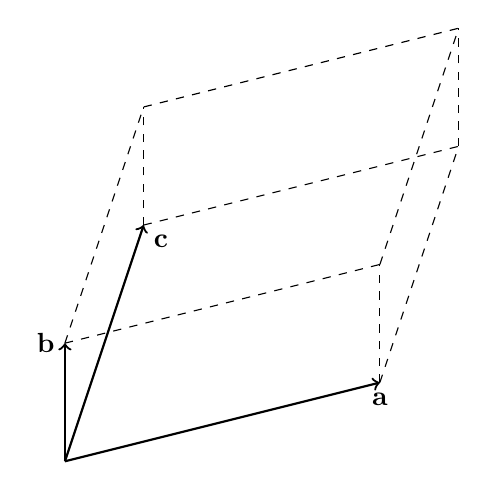
\begin{tikzpicture}
			\draw[thick,->] (0,0) -- (0,1.5) node[left] {$\vec{b}$};
			\draw[thick,->] (0,0) -- (4,1) node[below] {$\vec{a}$};
			\draw[thick,->] (0,0) -- (1,3) node[below right] {$\vec{c}$};
			\draw[dashed] (4,1) -- (4,2.5);
			\draw[dashed] (0,1.5) -- (4,2.5);
			\draw[dashed] (4,1) -- (5,4);
			\draw[dashed] (1,3) -- (5,4);
			\draw[dashed] (1,3) -- (1,4.5);
			\draw[dashed] (5,4) -- (5,5.5);
			\draw[dashed] (1,4.5) -- (5,5.5);
			\draw[dashed] (0,1.5) -- (1,4.5);
			\draw[dashed] (4,2.5) -- (5,5.5);
		\end{tikzpicture}
	\end{center}
	The area of the parallelogram (two dimensional front of this object) is given by,
	\[ \text{Area} = ||\vec{a} \times \vec{b} || \]
	and the volume of the parallelepiped (the whole three dimensional object) is given by,
	\[ \text{Volume} = \big| \vec{a} \cdot (\vec{b} \times \vec{c}) \big| \]
	Note that the absolute value bars are required since the quantity could be negative and volume isn't negative.


	\chapter{Three Dimensional Space}\normalsize
	
	In this chapter we will start to take a more detailed look at three dimensional space (3-D space or $ \R^3 $  ). This is a very important topic in Calculus III since a good portion of Calculus III is done in three (or higher) dimensional space.\\ \\
	We will be looking at the equations of graphs in 3-D space as well as vector valued functions and how we do calculus with them.  We will also be taking a look at a couple of new coordinate systems for 3-D space. 
	
	\section{The 3-D Coordinate System}
	
	Let's first get some basic notation out of the way. The 3-D coordinate system is often denoted by $ \R^3 $ . Likewise the 2-D coordinate system is often denoted by $ \R^2 $  and the 1-D coordinate system is denoted by $ \R $.  Also, as you might have guessed then a general $ n $ dimensional coordinate system is often denoted by $ \R^n $.\\ \\
	Next, let's take a quick look at the basic coordinate system.
	\begin{center}
		\tdplotsetmaincoords{70}{120}
		\begin{tikzpicture}[tdplot_main_coords]
		\def\BigSide{2.5}
		\def\SmallSide{1.5}
		\pgfmathsetmacro{\CalcSide}{\BigSide-\SmallSide}
		
		% The vertex at V
		\tdplotsetcoord{P}{sqrt(3)*\BigSide}{55}{45}
		
		\coordinate (sxl) at (\BigSide,\CalcSide,\BigSide);
		\coordinate (syl) at (\CalcSide,\CalcSide,\BigSide);
		\coordinate (szl) at (\CalcSide,\BigSide,\BigSide);
		
		\draw 
		(0,0,0) -- (Px)
		(0,0,0) -- (Py)
		(0,0,0) -- (Pz);
		\draw[->] 
		(Px) -- ++ (.25,0,0) node[anchor=north east]{$x$};
		\draw[->]
		(Py) -- ++(0,.25,0) node[anchor=north west]{$y$};
		\draw[->] 
		(Pz) -- ++(0,0,.25) node[anchor=south]{$z$};
		
		\draw[thick,dashed]
		(Pxz) -- (P) -- (Pyz);
		\draw[thick,dashed]
		(Pxy) -- (P);
		\node[label=below right:{$P=(x,y,z)$},fill,circle,inner sep=1.25pt] at (P) {};
		\node[label=above left:{$S=(x,0,z)$},fill,circle,inner sep=1.25pt] at (Pxz) {};
		\node[label=above right:{$R=(0,y,z)$},fill,circle,inner sep=1.25pt] at (Pyz) {};
		\node[label=below right:{$Q=(x,y,0)$},fill,circle,inner sep=1.25pt] at (Pxy) {};
		\end{tikzpicture}
	\end{center}
	This is the standard placement of the axes in this class.  It is assumed that only the positive directions are shown by the axes. If we need the negative axes for any reason we will put them in as needed. Also note the various points on this sketch.  The point $ P $ is the general point sitting out in 3-D space. If we start at $ P $ and drop straight down until we reach a $ z $-coordinate of zero we arrive at the point $ Q $.  We say that $ Q $ sits in the $ xy $-plane.  The $ xy $-plane corresponds to all the points which have a zero $ z $-coordinate. We can also start at $ P $ and move in the other two directions as shown to get points in the $ xz $-plane (this is $ S $ with a $ y $-coordinate of zero) and the $ yz $-plane (this is $ R $ with an $ x $-coordinate of zero).\\ \\
	Collectively, the $ xy $, $ xz $, and $ yz $-planes are sometimes called the coordinate planes. Also, the point $ Q $ is often referred to as the projection of $ P $ in the $ xy $-plane. Likewise, $ R $ is the projection of $ P $ in the $ yz $-plane and $ S $ is the projection of $ P $ in the $ xz $-plane.\\ \\
	Many of the formulas that you are used to working with in $ \R^2 $  have natural extensions in $ \R^3 $. For instance the distance between two points in $ \R^2 $ is given by,
	\[ d(P_1,P_2) = \sqrt{(x_2-x_1)^2+(y_2-y_1)^2} \]
	While the distance between any two points in $ \R^3 $ is given by,
	\[ d(P_1,P_2,P_3) = \sqrt{(x_2-x_1)^2+(y_2-y_1)^2+(z_2-z_1)^2} \]
	
	\section{Equations of Lines}
	
	So, before we get into the equations of lines we first need to briefly look at vector functions.  We’re going to take a more in depth look at vector functions later.  At this point all that we need to worry about is notational issues and how they can be used to give the equation of a curve.\\ \\
	A vector function is a function that takes one or more variables, one in this case, and returns a vector.  Note as well that a vector function can be a function of two or more variables.  However, in those cases the graph may no longer be a curve in space. We represent vectors with a bold face.\\ \\
	We want to write down the equation of a line in $ \R^3 $ and we will need a vector function to do this.  To see how we’'e going to do this let's think about what we need to write down the equation of a line in $ \R^2 $.  In two dimensions we need the slope $ (m) $ and a point that was on the line in order to write down the equation.\\ \\
	Suppose that we know a point that is on the line, $ P_0 = (x_0,y_0,z_0) $, and that $ \vec{v} = \langle a,b,c \rangle $  is some vector that is parallel to the line.  Note, in all likelihood,  will not be on the line itself.  We only need  to be parallel to the line.  Finally, let $ P=(x,y,z) $ be any point on the line.\\ \\
	Now, since our ``slope'' is a vector let's also represent the two points on the line as vectors.  We'll do this with position vectors. So, let $ \vec{r}_0 $ and $ \vec{r} $  be the position vectors for $ P_0 $ and $ P $ respectively. Also, let's define $ \vec{a} $ to be the vector with representation $ \vec{P_0P} $.\\ \\
	We now have the following sketch with all these points and vectors on it.
	\begin{center}
			\tdplotsetmaincoords{70}{120}
			\begin{tikzpicture}[tdplot_main_coords]
			\def\BigSide{2.5}
			\def\SmallSide{1.5}
			\pgfmathsetmacro{\CalcSide}{\BigSide-\SmallSide}
			% The vertex at V
			\tdplotsetcoord{P}{sqrt(3)*\BigSide}{55}{45}
			
			\coordinate (sxl) at (\BigSide,\CalcSide,\BigSide);
			\coordinate (syl) at (\CalcSide,\CalcSide,\BigSide);
			\coordinate (szl) at (\CalcSide,\BigSide,\BigSide);
			% Axes
			\draw 
			(0,0,0) -- (Px)
			(0,0,0) -- (Py)
			(0,0,0) -- (Pz);
			\draw[->] 
			(Px) -- ++ (1,0,0) node[anchor=north east]{$x$};
			\draw[->]
			(Py) -- ++(0,1,0) node[anchor=north west]{$y$};
			\draw[->] 
			(Pz) -- ++(0,0,1) node[anchor=south]{$z$};
			% Vectors
			\draw[thick,->] (0,0,0) -- (0,0.75,2);
			\draw[thick,->,draw=blue] (0,0,0) -- (1,2,1) node[below=1mm]{$\vec{v}$};
			\draw[thick,->,draw=blue] (0,0.75,2) -- (1,3.25,3.25);
			\draw[thick,->] (0,0,0) -- (1,3.25,3.25);
			% Points / Labels
			\draw  (0.5,1.625,1.625) node[below right] {$\vec{r}$};
			\draw  (0,0.6,1.5) node[left] {$\vec{r}_0$};
			\draw  (0,1.625,2.4) node[above] {$\vec{a}$};
			\node[label=above left:{$P_0$},fill,circle,inner sep=1.25pt] at (0,0.75,2) {};
			\node[label=right:{$P$},fill,circle,inner sep=1.25pt] at (1,3.25,3.25) {};
		\end{tikzpicture}
	\end{center}
	Now, we've shown the parallel vector, $ \vec{v} $, as a position vector but it doesn't need to be a position vector. It can be anywhere, a position vector, on the line or off the line, it just needs to be parallel to the line. Next, notice that we can write $ \vec{r} $ as follows,
	\[ \vec{r} = \vec{r}_0 + \vec{a} \]
	Now, notice that the vectors $ \vec{a} $ and $ \vec{v} $ are parallel. Therefore there is a number, $ t $, such that 
	\[ \vec{a} = t\vec{v} \]
	Combining these, we now have 
	\[ \vec{r} = \vec{r}_0 + t\vec{v} = \langle x_0,y_0,z_0 \rangle + t\langle a,b,c \rangle \]
	This is called the \textit{vector form of the equation of a line}. Notice that $ t\vec{v} $ will be a vector that lies along the line and tells us how far from the original point that we should we move.\\ \\
	There are several other forms of the equation of a line. To get the first alternate form let's start with the vector form and do a slight rewrite.
	\begin{align*}
		\vec{r} &= \langle x_0,y_0,z_0 \rangle + t\langle a,b,c \rangle\\
		\langle x,y,z  \rangle	&= \langle x_0 + ta,y_0 + tb,z_0 + tc \rangle 
	\end{align*}
	The only way for two vectors to be equal is for the components to be equal. In other words,
	\begin{align*}
		x &= x_0 + ta\\
		y &= y_0 + tb\\
		z &= z_0 + tc
	\end{align*}
	This set of equations are called \textit{parametric form of the equation of a line}. To get a point on the line all we do is pick a $ t $ and plug into either form of the line. In the vector form of the line we get a position vector for the point and in the parametric form we get the actual coordinates of the point. If we assume that $a$, $b$, and $c$ are all non-zero numbers we can solve each of the equations in the parametric form of the line for $t$. We can then set all of them equal to each other since $t$ will be the same number in each. Doing this gives the following,
	\[ \frac{x - x_0}{a} = \frac{y - y_0}{b} = \frac{z - z_0}{c} \]
	This is called the \textit{symmetric equation of the line}.
	
	\section{Equations of Planes}
	
	Let's start assuming that we know a point on the plane, $ P_0 = (x_0,y_0,z_0) $. Let's also suppose that we have a vector that is orthogonal (perpendicular) to the plane, $ \vec{n} = \langle a,b,c \rangle $. This is called the \textit{normal vector}. Now, assume that $ P = (x,y,z) $ is any point in the plane. Finally, we'll let $ \vec{r} $ and $ \vec{r}_0 $ be the position vectors for $ P $ and $ P_0 $ respectively. Here's the sketch,
	\begin{center}
		\tdplotsetmaincoords{70}{110}
		\begin{tikzpicture}[scale=3,tdplot_main_coords]
    	\draw[thick,->] (0,0,0) -- (1,0,0) node[anchor=north east]{$x$};
    	\draw[thick,->] (0,0,0) -- (0,2,0) node[anchor=north west]{$y$};
    	\draw[thick,->] (0,0,0) -- (0,0,1.75) node[anchor=south]{$z$};

    	% plane
        \fill[cyan!50,opacity=0.6] (0,0,1.5) -- (2,0,1.5) -- (2,1,1) -- (0,1,1) -- (0,0,1.5);

        % vec r
        \draw[thick,->,opacity=0.6] (0,0,0) -- (0.5,0,1);
        \draw[thick] (0,0,0) -- (0.25,0,0.5);

        % vec r0
        \draw[thick,->,opacity=0.6] (0,0,0) -- (0,0.5,0.75);
        \draw[thick] (0,0,0) -- (0,0.18,0.27);

        % vec r-r0
        \draw[thick,->,draw=red] (0,0.5,0.75) -- (0.5,0,1);

        % points / nodes
        \node[label=above:{$P$},fill,circle,inner sep=1.25pt] at (0.5,0,1) {};
        \node[label=above:{$P_0$},fill,circle,inner sep=1.25pt] at (0,0.5,0.75) {};
        \draw (0,0.2,0.875) node[below=3mm] {$\vec{r} - \vec{r}_0$};
        \draw (0.25,0,0.5) node[below left] {$\vec{r}$};
        \draw (0,0.25,0.375) node[right] {$\vec{r}_0$};

        % normal vec
        \draw[thick,->] (0,0.5,1.1) -- (0,0.65,1.3) node[above] {$\vec{n}$};


		\end{tikzpicture}
	\end{center}
	Notice that the vector $ \vec{r} - \vec{r}_0 $ lies completely on the plane. Now, because $\vec{n}$ is orthogonal to the plane, it's also orthogonal to any vector that lies in the plane. In particular, it's orthogonal ot $\vec{r} - \vec{r}_0$. Recall from the Dot Product that two orthogonal vectors will have a dot product of zero. In other words,
	\[ \vec{n} \cdot (\vec{r} - \vec{r}_0) = 0 \qquad \Rightarrow \qquad \vec{n} \cdot \vec{r} = \vec{n} \cdot \vec{r}_0 \]
	This is called the \textit{vector equation of the plane}.\\ \\
	A slightly more useful form of the equation is as follows. Start with the first form of the vector equation and write down a vector for the difference.
	\begin{align*}
		\langle a,b,c \rangle \cdot \left( \langle x,y,z \rangle - \langle x_0,y_0,z_0 \rangle \right) &= 0\\
		\langle a,b,c \rangle \cdot \langle x-x_0,y-y_0,z-z_0 \rangle &= 0\
	\end{align*}
	Now compute the dot product to get,
	\[ a(x-x_0) + b(y-y_0) + c(z-z_0) = 0 \]
	This is called the \textit{scalar equation of the plane}. Often this will be written as,
	\[ ax + by + cz = d \]
	where $d=ax_0 + by_0 + cz_0$

	\section{Quadric Surfaces}

	Quadric surfaces are the graphs of any equation that can be put into the general form
	\[ Ax^2 + By^2 + Cz^2 + Dxy + Exz + Fyz + Gx + Hy + Iz + J = 0 \]
	where $A,\ldots,J$ are constants. Now, there is no way we can possibly list all of them, but there are some standard equations so here is a table of some of the more common quadric surfaces.\\ \\
	
	\begin{table}[ht]
		\centering
		\begin{tabular}{*{4}{m{0.25\textwidth}}}
			Name & Equation &  Graph \\ \hline
			Ellipsoid & $ \displaystyle{\frac{x^2}{a^2} + \frac{y^2}{b^2} + \frac{z^2}{c^2}=1} $ &  \begin{center}\includegraphics[scale=.25]{image001.png}\end{center}\\ \hline
			Cone & $ \displaystyle{\frac{x^2}{a^2} + \frac{y^2}{b^2} = \frac{z^2}{c^2}} $ & \begin{center} \includegraphics[scale=0.25]{image002.png}\end{center}\\ \hline
			Cylinder & $ \displaystyle{\frac{x^2}{a^2} + \frac{y^2}{b^2}=1} $ & \begin{center} \includegraphics[scale=0.25]{image003.png} \end{center} \\ \hline
			Hyperboloid of One Sheet & $ \displaystyle{\frac{x^2}{a^2} + \frac{y^2}{b^2} - \frac{z^2}{c^2}=1} $ & \begin{center} \includegraphics[scale=0.25]{image004.png} \end{center} \\ \hline
		\end{tabular}
	\end{table}

	\begin{table}[ht]
		\centering
		\begin{tabular}{*{4}{m{0.25\textwidth}}}
			 \\ \hline
			Hyperboloid of Two Sheets & $ \displaystyle{-\frac{x^2}{a^2} + \frac{y^2}{b^2} + \frac{z^2}{c^2}=1} $ & \begin{center} \includegraphics[scale=0.25]{image005.png} \end{center} \\ \hline
			Elliptic Paraboloid & $ \displaystyle{\frac{x^2}{a^2} + \frac{y^2}{b^2} = \frac{z}{c}} $ & \begin{center} \includegraphics[scale=0.25]{image006.png} \end{center} \\ \hline
			Hyperbolic Paraboloid & $ \displaystyle{\frac{x^2}{a^2} - \frac{y^2}{b^2} = \frac{z}{c}} $ & \begin{center} \includegraphics[scale=0.25]{image007.png} \end{center} \\ \hline
		\end{tabular}
	\end{table}

\newpage

	\section{Vector Functions}

	A vector function is a function that takes one or more variables and returns a vector. A vector function of a single variable in $\R^2$ and $\R^3$ have the form,
	\[ \vec{r}(t) = \langle f(t),g(t) \rangle \qquad \vec{r}(t) = \langle f(t),g(t),h(t) \rangle \]
	where $f(t)$, $g(t)$, and $h(t)$ are called the \textit{component functions}.\\ \\
	The domain of a vector function is the set of all $t$'s for which all the component functions are defined.\\ \\
	Any vector function can be broken down into a set of parametric equations that represent the same graph. In general, the two dimensional vector function, $ \vec{r}(t) =  \langle f(t),g(t) \rangle $, can be broken down into the parametric equations,
	\[ x = f(t) \qquad y = g(t) \]
	Likewise, a three dimensional vector function, $ \vec{r}(t) = \langle f(t),g(t),h(t) \rangle $, can be broken down into the parametric equations,
	\[ x = f(t) \qquad y = g(t) \qquad z = h(t) \]
	
	\section{Calculus with Vector Functions}
	
	Given the vector function $ \vec{r}(t) = \langle f(t),g(t),h(t) \rangle $, the limit of $ \vec{r}(t) $ as it approaches a value $ \alpha $, is
	\begin{align*}
		\lim_{t \to \alpha} \vec{r}(t) &= \lim_{t \to \alpha} \big\langle f(t),g(t),h(t) \big\rangle\\
		&= \bigg\langle \lim_{t \to \alpha} f(t), \lim_{t \to \alpha} g(t), \lim_{t \to \alpha} h(t) \bigg\rangle\\
		&= \lim_{t \to \alpha} f(t)\,\uvec{\i} + \lim_{t \to \alpha} g(t)\,\uvec{\j} + \lim_{t \to \alpha} h(t)\,\uvec{k}
	\end{align*}
	So, all that we do is take the limit of each of the component's functions and leave it as a vector.\\ \\
	Derivatives are very similar, 
	\begin{align*}
		\vec{r}'(t) &= \langle f'(t),g'(t),h'(t) \rangle\\
					&= f'(t)\uvec{\i} + g'(t)\uvec{\j} + h'(t)\uvec{k}
	\end{align*}
	Most of the basic facts that we know about derivatives still hold. Given two vectors $ \vec{u} $, $ \vec{v} $, a real valued function $ f(t) $, and a real number $ c $, we have the following properties
	\begin{align*}
		& \frac{d}{dt}(\vec{u} + \vec{v}) = \vec{u}' + \vec{v}'\\
		& \frac{d}{dt}(c\vec{u}) = c\vec{u}'\\
		& \frac{d}{dt}(f(t)\vec{u}) = f(t)\vec{u}' + f'(t)\vec{u}\\
		& \frac{d}{dt}(\vec{u} \cdot \vec{v}) = \vec{u}\vec{v}' + \vec{u}'\vec{v}\\
		& \frac{d}{dt}(\vec{u} \cdot \vec{v}) = \vec{u} \cdot \vec{v}' + \vec{u}' \cdot \vec{v}\\
		& \frac{d}{dt}(\vec{u} \times \vec{v}) = \vec{u} \times \vec{v}' + \vec{u}' \times \vec{v}\\
		& \frac{d}{dt}(\vec{u}(f(t))) = f'(t)\vec{u}'(f(t))
	\end{align*}
	Before getting to integration we need to define what a smooth curve is. A \textit{smooth curve} is any curve for which $ \vec{r}(t) $  is continuous and $ \vec{r}(t) \neq 0 $ for any $ t $ except possibly at the endpoints. A helix is a smooth curve, for example.\\ \\
	Finally, the integral of a vector function is defined as
	\begin{align*}
		\int \vec{r}(t) &= \bigg\langle \int f(t)\,dt. \int g(t)\,dt, \int h(t)\,dt \bigg\rangle + \vec{c}\\
		&= \int f(t)\,dt\,\uvec{\i} + \int g(t)\,dt\,\uvec{\j} + \int h(t)\,dt\,\uvec{k} + \vec{c}
	\end{align*}
	and the following for definite integrals
	\begin{align*}
		\int\limits_{\alpha}^{\beta} \vec{r}(t)\,dt &= \bigg\langle \int\limits_{\alpha}^{\beta} f(t)\,dt. \int\limits_{\alpha}^{\beta} g(t)\,dt, \int\limits_{\alpha}^{\beta} h(t)\,dt \bigg\rangle\\
		&= \int\limits_{\alpha}^{\beta} f(t)\,dt\,\uvec{\i} + \int\limits_{\alpha}^{\beta} g(t)\,dt\,\uvec{\j} + \int\limits_{\alpha}^{\beta} h(t)\,dt\,\uvec{k}
	\end{align*}
	
	\section{Tangent, Normal, and Binormal Vectors}
	
	In the past we've used the fact that the derivative of a function was the slope of the tangent line.  With vector functions we get exactly the same result, with one exception.\\ \\
	Given the vector function, $ \vec{r}(t) $, we call $ \vec{r}'(t) $ the \textit{tangent vector} provided it exists and provided $ \vec{r}(t) \neq \vec{0} $. The tangent line to $ \vec{r}(t) $ at $ P $ is then the line that passes through the point $ P $ and is parallel to the tangent vector, $ \vec{r}'(t) $. Also, provided $ \vec{r}'(t) \neq \vec{0} $, the \textit{unit tangent vector} to the curve is given by,
	\[ \vec{T}(t) = \frac{\vec{r}'(t)}{|| \vec{r}'(t) ||} \]
	While, the components of the unit tangent vector can be somewhat messy on occasion there are times when we will need to use the unit tangent vector instead of the tangent vector.\\ \\
	The unit normal is orthogonal (or normal, or perpendicular) to the unit tangent vector and hence to the curve as well. The \textit{unit normal vector} is given by,
	\[ \vec{N}(t) = \frac{\vec{T}'(t)}{|| \vec{T}'(t) ||} \]
	Next is the binormal vector. The binormal vector is defined to be,
	\[ \vec{B}(t) = \vec{T}(t) \times \vec{N}(t) \]
	Because the binormal vector is defined to be the cross product of the unit tangent and unit normal vector we then know that the binormal vector is orthogonal to both the tangent vector and the normal vector.
	
	\section{Arc Length with Vector Functions}
	
	In this section we'll recast an old formula into terms of vector functions. We want to determine the length of a vector function,
	\[ \vec{r}(t) = \langle f(t),g(t),h(t) \rangle \]
	on the interval $ \alpha \leq t \leq \beta $. We actually already know how to do this. Recall that we can write the vector function into the parametric form,
	\[ x = f(t) \qquad y = g(t) \qquad z = h(t) \]
	Also, recall that with two dimensional parametric curves the arc length is given by,
	\[ L = \int\limits_{\alpha}^{\beta} \sqrt{(f'(t))^2 + (g'(t))^2 }\,dt \]
	There is a natural extension of this to three dimensions.  So, the length of the curve $ \vec{r}(t) $ on the interval $ \alpha \leq t \leq \beta $ is,
	\[ L = \int\limits_{\alpha}^{\beta} \sqrt{(f'(t))^2 + (g'(t))^2 + (h'(t))^2}\,dt \]
	There is a nice simplification that we can make for this. Notice that the integrand is nothing more than the magnitude of the tangent vector,
	\[ || \vec{r}'(t) || = \sqrt{(f'(t))^2 + (g'(t))^2 + (h'(t))^2} \]
	Therefore, the arc length can be written as,
	\[ L = \int\limits_{\alpha}^{\beta} || \vec{r}'(t)||\,dt \]
	
	
	\section{Curvature}
	
	Curvature is the measure of how fast a curve is changing direction at a given point. The formal definition of curvature is,
	\[ \kappa = \bigg\lvert \frac{d\vec{T}}{ds} \bigg\rvert \]
	where $ \vec{T} $ is the unit tangent vector and $ s $ is the arc length. In general the formal definition of the curvature is not easy to use so there are two alternate formulas that we can use.  Here they are.
	\[ \kappa = \frac{||\vec{T}'(t)||}{||\vec{r}'(t)||} \qquad \kappa = \frac{||\vec{r}'(t) \times \vec{r}''(t)||}{|| \vec{r}'(t) ||^3} \]
	These may not be particularly easy to deal with either, but at least we don’t need to reparameterize the unit tangent.\\ \\
	There is a special case that we can look at. Suppose we have a curve given by $ y = f(x) $ and we want to find its curvature. We can write it as a standard vector function in the form
	\[ \vec{r}(t) = x\,\uvec{\i} + f(x)\,\uvec{\j} \]
	If we then use the second formula for the curvature we will arrive at the following formula for the curvature.
	\[ \kappa = \frac{\big|f'(x)\big|}{\big( 1 + (f'(x))^2 \big)^{3/2}} \]
	
	\section{Velocity and Acceleration}
	
	From Calculus I we know that given the position function of an object that the velocity of the object is the first derivative of the position function and the acceleration of the object is the second derivative of the position function. So given an object's position vector $ \vec{r}(t) $ the object's velocity and acceleration are given by 
	\[ \vec{v}(t) = \vec{r}'(t) \qquad \vec{a}(t) = \vec{r}''(t) \]
	Notice that the velocity and acceleration are going to be vector functions as well.
	
	\section{Cylindrical Coordinates}
	
	 The last two sections of this chapter we’ll be looking at some alternate coordinate systems for three dimensional space. As with two dimensional space the standard $ (x,y,z) $ coordinate system is called the Cartesian coordinate system.\\ \\
	 Cylindrical coordinates are fairly simple as it is nothing more than extending polar coordinates into $ \R^3 $. Not only is it an extension of polar coordinates, but we extend it into the third dimension just as we extend Cartesian coordinates into the third dimension.  All that we do is add a $ z $ on as the third coordinate. The $ r $ and $ \theta $ are the same as with polar coordinates. Here is a sketch.
	 
	 \begin{center}
	 	\tdplotsetmaincoords{70}{120}
	 	\begin{tikzpicture}[tdplot_main_coords]
	 	\def\BigSide{2.5}
	 	\def\SmallSide{1.5}
	 	\pgfmathsetmacro{\CalcSide}{\BigSide-\SmallSide}
	 	
	 	% The vertex at V
	 	\tdplotsetcoord{P}{sqrt(3)*\BigSide}{55}{45}
	 	
	 	\coordinate (sxl) at (\BigSide,\CalcSide,\BigSide);
	 	\coordinate (syl) at (\CalcSide,\CalcSide,\BigSide);
	 	\coordinate (szl) at (\CalcSide,\BigSide,\BigSide);
	 	
	 	\draw[->] (0,0,0) -- (2.5,0.25,0) node[below] {$x$};
	 	\draw[->] (0,0,0) -- (0,4,0) node[right] {$y$};
		\draw[->] (0,0,0) -- (0,0,3) node[above] {$z$};
		
		\draw[dashed] (0,0,0) -- (1,3,0);
		\draw[dashed] (1,3,0) -- (1,3,3);
		\draw[->] (1,0.1) to [bend right] (0.37,1);
		
		\node[label=above:{$(x,y,z) = (r,\theta,z)$},fill,circle,inner sep=1.25pt] at (1,3,3) {};
		\draw (1.7,1,0) node[right] {$\theta$};
		\draw (0.6,2,0) node[below=1mm] {$r$};
		\draw (0.5,2.75,1.5) node[right] {$z$};
	 	\end{tikzpicture}
	\end{center}
 	The conversions for $ x $ and $ y $ are the same conversions that we used back when we were looking at polar coordinates.  So, if we have a point in cylindrical coordinates the Cartesian coordinates can be found by using the following conversions
 	\begin{align*}
 		x &= r\cos(\theta)\\
 		y &= r\sin(\theta)\\
 		z &= z
 	\end{align*}
 	The third equation is just an acknowledgement that the z-coordinate of a point in Cartesian and polar coordinates is the same. Likewise, if we have a point in Cartesian coordinates the cylindrical coordinates can be found by using the following conversions
 	\begin{align*}
 		r &= \sqrt{x^2 + y^2} \qquad \text{or} \qquad r^2 = x^2 + y^2\\
 		\theta &= \tan^{-1}\left( \frac{y}{x} \right)\\
 		z &= z
 	\end{align*}
 	
 	\section{Spherical Coordinates}
 	
 	Let's start with a sketch
	
	\begin{center}
		\tdplotsetmaincoords{70}{120}
		\begin{tikzpicture}[tdplot_main_coords]
			\draw[->] (0,0,0) -- (4,0,0) node[left] {$x$};
			\draw[->] (0,0,0) -- (0,4,0) node[right] {$y$};
			\draw[->] (0,0,0) -- (0,0,4) node[above] {$z$};
			
			\node[label=above:{$(x,y,z) = (\rho,\theta,\phi)$},fill,circle,inner sep=1.25pt] at (2,4,3) {};
			
			\draw (0,0,0) -- (2,4,3);
			\draw[dashed] (0,0,0) -- (2,4,0);
			\draw[dashed] (2,4,0) -- (2,4,3);
			
			\draw[->] (1,0) to [bend right] (0.6,1);
			\draw[->] (0,0,1) to [bend left] (0,1,0.75);
			
			\draw (0,0.5,1) node[above] {$\phi$};
			\draw (0.7,0.5,0) node[below=2mm] {$\theta$};
			\draw (1,2,1.5) node[above] {$\rho$};
			\draw (1,2.5) node[below=2mm] {$r$};
			\draw (1,3.5,1.5) node[right] {$z$};
		\end{tikzpicture}
	\end{center}
	Spherical coordinates consist of the following three quantities.\\ \\
	First there is $ \rho $. This is the distance from the origin to the point, we require $ \rho \geq 0 $.\\ \\
	Next there is $ \theta $. This is the same angle from polar/cylindrical coordinates. It is the angle between the positive $ x $-axis and the line denoted by $ r $(which is also the same $ r $ in polar/cylindrical coordinates).\\ \\
	Finally there is $ \phi $. This is the angle between the positive $ z $-axis and the line from the origin to the point. We will require $ 0 \leq \phi \leq \pi $.\\ \\
	So, given a point in spherical coordinates the cylindrical coordinates of the point will be,
	\begin{align*}
		r &= \rho\sin(\phi)\\
		\theta &= \theta\\
		z &= \rho\cos(\phi)
	\end{align*}
	Note as well that,
	\begin{align*}
		r^2 + z^2 &= \rho^2\cos^2(\phi) + \rho^2\sin^2(\phi)\\
		&= \rho^2(\cos^2(\phi) + \sin^2(\phi)\\
		&= \rho^2
	\end{align*}
	
	\chapter{Partial Derivatives}
	
	In Calculus III we will extend our knowledge of calculus into functions of two or more variables. Despite the fact that this chapter is about derivatives we will start out the chapter with a section on limits of functions of more than one variable. In the remainder of this chapter we will be looking at differentiating functions of more than one variable. As we will see, while there are differences with derivatives of functions of one variable, if you can do derivatives of functions of one variable you shouldn’t have any problems differentiating functions of more than one variable.
	
	\section{Limits}
	
	In this section we will take a look at limits involving functions of more than one variable. In fact, we will concentrate mostly on limits of functions of two variables, but the ideas can be extended out to functions with more than two variables. Before getting into this let's briefly recall how limits of functions of one variable work. We say that,
	\[ \lim_{x \to \alpha} f(x) = L \]
	provided that 
	\[ \lim_{x \to \alpha^+} f(x) = \lim_{x \to \alpha^-} f(x) = L \]
	In other words, we will have $\displaystyle{\lim_{x \to \alpha} f(x)} = L $ provided $ f(x) $ approaches $ L $ as we move in towards $ x = \alpha $  (without letting $ x = \alpha $) from both sides. Now, notice that in this case there are only two paths that we can take as we move in towards $ x = \alpha $. We can either move in from the left or we can move in from the right. Then in order for the limit of a function of one variable to exist the function must be approaching the same value as we take each of these paths in towards $ x = \alpha $.\\ \\
	With functions of two variables we will have to do something similar, except this time there is (potentially) going to be a lot more work involved. Let's first address the notation and get a feel for just what we're going to be asking for in these kinds of limits. We will be asking to take the limit of the function $ f(x,y) $ as $ x $ approaches $ a $ and as $ y $ approaches $ b $. Here is the standard notation,
	\[ \lim_{(x,y) \to (a,b)} f(x,y) \]
	 In taking a limit of a function of two variables we are really asking what the value of $ f(x,y) $ is doing as we move the point $ (x,y) $ in closer and closer to the point $ (a,b) $ without actually letting it be $ (a,b) $.\\ \\
	 Just like with limits of functions of one variable, in order for this limit to exist, the function must be approaching the same value regardless of the path that we take as we move in towards $ (a,b) $. The problem that we are immediately faced with is that there are literally an infinite number of paths that we can take as we move in towards $ (a,b) $. Here are a few examples of paths that we could take.
	 
	 \begin{center}
	 	\begin{tikzpicture}
	 		\draw (0,0) -- (5,0) node[below] {$x$};
	 		\draw (1,-0.25) -- (1,4) node[left] {$y$};
	 		\draw (2.5,0) node[below] {$a$};
	 		\draw (1,1.5) node[left] {$b$};
	 		
			\node[fill,circle,inner sep=1.25pt] at (2.5,1.5) {};
			
			\draw[dashed] (2.5,0) -- (2.5,1.5);
			\draw[dashed] (1,1.5) -- (2.5,1.5);
			
			\draw[->] (1.3,1) -- (2.4,1.4);
			\draw[->] (3,3) -- (2.6,1.6);
			\draw[->] (3.5,0.25) -- (2.6,1.4);
			\draw[->] (1.1,0.2) to [bend right] (2.45,1.3);
			\draw[->] (1.5,3.8) to [bend left] (2.45,1.6);
			\draw[->] (4,2) to [bend left] (2.6,1.5);
	 	\end{tikzpicture}
	 \end{center}
 	In other words, to show that a limit exists we would technically need to check an infinite number of paths and verify that the function is approaching the same value regardless of the path we are using to approach the point. The way we approach this is to use one of the main ideas from Calculus I limits.\\ \\
 	\textbf{Definition}\\
 	A function $ f(x,y) $ is continuous at the point $ (a,b) $ if,
 	\[ \lim_{(x,y) \to (a,b)} f(x,y) = f(a,b) \]
 	From a graphical standpoint this definition means the same thing as it did when we first saw continuity in Calculus I. A function will be continuous at a point if the graph doesn't have any holes or breaks at that point.\\ \\
 	\textbf{Example}\\
 	\[ \lim_{(x,y) \to (0,0)} \frac{x^2 y^2}{x^4 + 3y^4} \]
	Now, in this case the function is not continuous at the point in question and so we can't just plug in the point. So, since the function is not continuous at the point there is at least a chance that the limit doesn't exist. If we could find two different paths to approach the point that gave different values for the limit then we would know that the limit didn't exist. Two of the more common paths to check are the $ x $ and $ y $-axis so let's try those.\\ \\
	So, let's see what happens along the $ x $-axis. If we are going to approach $ (0,0) $ along the $ x $-axis we can take advantage of the fact that that along the $ x $-axis we know that $ y = 0 $. This means that, along the $ x $-axis, we will plug in $ y = 0 $ into the function and then take the limit as $ x $ approaches zero.
	\[ \lim_{(x,y) \to (0,0)} \frac{x^2 y^2}{x^4 + 3y^4} = \lim_{(x,0) \to (0,0)} \frac{x^2 (0)^2}{x^4 + 3(0)^4} = \lim_{(x,0) \to (0,0)} 0 = 0 \]
	So, along the $ x $-axis the function will approach zero as we move in towards the origin. Now, let's try the $ y $-axis. Along this axis we have $ x = 0 $ and so the limit becomes,
	\[ \lim_{(x,y) \to (0,0)} \frac{x^2 y^2}{x^4 + 3y^4} = \lim_{(0,y) \to (0,0)} \frac{(0)^2 y^2}{(0)^4 + 3y^4} = \lim_{(0,y) \to (0,0)} 0 = 0  \]
	So, the same limit along two paths. Don't misread this. This does NOT say that the limit exists and has a value of zero. This only means that the limit happens to have the same value along two paths. Let's take a look at a third fairly common path to take a look at. In this case we'll move in towards the origin along the path $ y =mx $, where $ m $ is just a number. This is what we meant previously about relating $ x $ and $ y $ through a function. To do this we will replace all the $ y $'s with $ mx $'s and then let $ mx $ approach zero. Let's take a look at this limit.
	\[ \lim_{(x,y) \to (0,0)} \frac{x^2 y^2}{x^4 + 3y^4} = \lim_{(x,mx) \to (0,0)} \frac{x^2 (mx)^2}{x^4 + 3(mx)^4} = \lim_{(x,mx) \to (0,0)} \frac{m^2 x^4}{x^4 + 3m^4 x^4} = \lim_{(x,mx) \to (0,0)} \frac{m^2}{1 + 3m^4}  \]
	Since we're just left with $ m $'s and we know that $ m $ can be any number, this means that that we will get a different value with each $ m $ we pick. So since the value of the limit is different from the two previous paths we chose, the limit does not exist.
	
	\section{Partial Derivatives}
	
	Recall that given a function of one variable, $ f(x) $, the derivative, $ f'(x) $, represents the rate of change of the function as $ x $ changes. This is an important interpretation of derivatives and we are not going to want to lose it with functions of more than one variable. The problem with functions of more than one variable is that there is more than one variable. In other words, what do we do if we only want one of the variables to change, or if we want more than one of them to change? In fact, if we're going to allow more than one of the variables to change there are then going to be an infinite amount of ways for them to change. For instance, one variable could be changing faster than the other variable(s) in the function. Notice as well that it will be completely possible for the function to be changing differently depending on how we allow one or more of the variables to change. \\ \\
	Let's start with the function $ f(x,y) = 2x^2 y^3 $ and let's determine the rate at which the function is changing at a point, $ (a,b) $, if we hold $ y $ fixed and allow $ x $ to vary and if we hold $ x $ fixed and allow $ y $ to vary.\\ \\ 
	We'll start by looking at the case of holding $ y $ fixed and allowing $ x $ to vary.  Since we are interested in the rate of change of the function at $ (a,b) $ and are holding $ y $ fixed this means that we are going to always have $ y = b $ (if we didn't have this then eventually $ y $ would have to change in order to get to the point…). Doing this will give us a function involving only $ x $’s and we can define a new function as follows,
	\[ g(x) = f(x,b) = 2x^2b^3 \]
	Now, this is a function of a single variable and at this point all that we are asking is to determine the rate of change of $ g(x) $ at $ x = a $. In other words, we want to compute $ g'(a) $ and since this is a function of a single variable we already know how to do that. Here is the rate of change of the function at $ (a,b) $ if we hold $ y $ fixed and allow $ x $ to vary.
	\[ g'(a) = 4ab^3 \]
	We will call $ g'(a) $ the \textit{partial derivative} of $ f(x,y) $ with respect to $ x $ at $ (a,b) $ and we will denote it in the following way,
	\[ f_x(a,b) = 4ab^3 \]
	Now, let's do it the other way. We will now hold $ x $ fixed and allow $ y $ to vary. We can do this in a similar way. Since we are holding $ x $ fixed it must be fixed at $ x = a $ and so we can define a new function of $ y $ and then differentiate this as we've always done with functions of one variable.
	\[ h(y) = f(a,y) = 2a^2y^3 \quad \Rightarrow \quad  h'(b) = 6a^2 b^2 \]
	In this case we call $ h'(b) $ the \textit{partial derivative} of $ f(x,y) $ with respect to $ y $ at $ (a,b) $ and we denote it as follows,
	\[ f_y(a,b) = 6a^2b^2 \]
	Now, as this quick example has shown taking derivatives of functions of more than one variable is done in pretty much the same manner as taking derivatives of a single variable. To compute $ f_x(x,y) $ all we need to do is treat all the $ y $'s as constants (or numbers) and then differentiate the $ x $'s as we've always done. Likewise, to compute $ f_y(x,y) $ we will treat all the $ x $'s as constants and then differentiate the $ y $'s as we are used to doing.\\ \\
	Since we can think of the two partial derivatives above as derivatives of single variable functions it shouldn't be too surprising that the definition of each is very similar to the definition of the derivative for single variable functions. Here are the formal definitions of the two partial derivatives we looked at above.
	\[ f_x(x,y) = \lim_{h \to 0} \frac{f(x+h,y) - f(x,y)}{h} \qquad f_y(x,y) = \lim_{h \to 0} \frac{f(x,y+h) - f(x,y)}{h} \]
	Now let's take a quick look at some of the possible alternate notations for partial derivatives. Given the function $ z = f(x,y) $ the following are all equivalent notations,
	\begin{align*}
		& f_x(x,y) = f_x = \frac{\partial f}{\partial x} = z_x = \frac{\partial z}{\partial x} = D_x f\\
		& f_y(x,y) = f_y = \frac{\partial f}{\partial y} = z_y = \frac{\partial z}{\partial y} = D_y f
	\end{align*}
	
	\section{Higher Order Partial Derivatives}
	
	Just as we had higher order derivatives with functions of one variable we will also have higher order derivatives of functions of more than one variable. However, this time we will have more options since we do have more than one variable.\\ \\
	Consider the case of a function of two variables, $ f(x,y) $ since both of the first order partial derivatives are also functions of $ x $ and $ y $ we could in turn differentiate each with respect to $ x $ or $ y $. This means that for the case of a function of two variables there will be a total of four possible second order derivatives. Here they are and the notations that we'll use to denote them.
	\begin{align*}
		& (f_x)_x = f_{xx} = \frac{\partial}{\partial x} \left(\frac{\partial f}{\partial x}\right) = \frac{\partial^2 f}{\partial x^2}\\
		& (f_x)_y = f_{xy} = \frac{\partial}{\partial y} \left(\frac{\partial f}{\partial x}\right) = \frac{\partial^2 f}{\partial y \, \partial x}\\
		& (f_y)_x = f_{yx} = \frac{\partial}{\partial x} \left(\frac{\partial f}{\partial y}\right) = \frac{\partial^2 f}{\partial x \, \partial y}\\
		& (f_y)_y = f_{yy} = \frac{\partial}{\partial y} \left(\frac{\partial f}{\partial y}\right) = \frac{\partial^2 f}{\partial y^2}
	\end{align*}
	The second and third second order partial derivatives are often called \textit{mixed partial derivatives} since we are taking derivatives with respect to more than one variable. Note as well that the order that we take the derivatives in is given by the notation for each these. If we are using the subscripting notation, e.g. $ f_{xy} $, then we will differentiate from left to right. In other words, in this case, we will differentiate first with respect to $ x $ and then with respect to $ y $. With the fractional notation, e.g. $ \partial^2 f / \partial y \, \partial x $, it is the opposite. In these cases we differentiate moving along the denominator from right to left. So, again, in this case we differentiate with respect to $ x $ first and then $ y $.
	
	\section{Differentials}
	
	 Just like we had differentials for functions of one variable we also have them for functions of more than one variable. Also, as we've already seen in previous sections, when we move up to more than one variable things work pretty much the same, but there are some small differences. Given the function $ z = f(x,y) $ the differential $ dz $ or $ df $ is given by,
	 \[ dz = f_x\,dx + f_y\,dy \qquad \text{or} \qquad df = f_x\,dx + f_y\,dy \]
	 There is a natural extension to functions of three or more variables. For instance, given the function $ w=g(x,y,z) $ the differential is given by,
	 \[ dw = g_x\,dx + g_y\,dy + g_z\,dz \]
	 
	\section{Chain Rule}
	 	
	Recall the chain rule for a single variable function $ F = f(g(x)) $,
	\[ F' = f'(g(x)) g'(x) \]
	There is an alternate notation however that while probably not used much in Calculus I is more convenient at this point because it will match up with the notation that we are going to be using in this section. If $ y = f(x) $ and $ x = g(t) $ then
	\[ \frac{dy}{dt} = \frac{dy}{dx} \frac{dx}{dt} \]
	Notice that the derivative $ dy/dt $ really does make sense here since if we were to plug in for $ x $ then $ y $ really would be a function of $ t $. One way to remember this form of the chain rule is to note that if we think of the two derivatives on the right side as fractions the $ dx $'s will cancel to get the same derivative on both sides.\\ \\
	We will be looking at two distinct cases prior to generalizing the whole idea out. Let's look at the first case\\ \\
	\textbf{Case I.} $ z = f(x,y) $, $ x = g(t) $, $ y= h(t) $. Compute $ dz/dt $.\\ \\
	This case is analogous to the standard chain rule from Calculus I that we looked at above. In this case we are going to compute an ordinary derivative since $ z $ really would be a function of $ t $ only if we were to substitute in for $ x $ and $ y $. The chain rule for this case is, 
	\[ \frac{dz}{dt} = \frac{\partial f}{\partial x} \frac{dx}{dt} + \frac{\partial f}{\partial y} \frac{dy}{dt} \]
	So, basically what we're doing here is differentiating $ f $ with respect to each variable in it and then multiplying each of these by the derivative of that variable with respect to $ t $. The final step is to then add all this up.\\ \\ 
	\textbf{Case II.} $ z = f(x,y) $, $ x = g(s,t) $, $ y = h(s,t) $. Compute $ \partial z / \partial s $ and $ \partial z / \partial t $.\\ \\
	In this case if we were to substitute in for $ x $ and $ y $ we would get that $ z $ is a function of $ s $ and $ t $ and so it makes sense that we would be computing partial derivatives here and that there would be two of them. Here is the chain rule for both of these cases.
	\[ \frac{\partial z}{\partial s} = \frac{\partial f}{\partial x} \frac{\partial x}{\partial s} + \frac{\partial f}{\partial y} \frac{\partial y}{\partial s} \qquad \quad  \frac{\partial z}{\partial t} =  \frac{\partial f}{\partial x} \frac{\partial x}{\partial t} + \frac{\partial f}{\partial y} \frac{\partial y}{\partial t} \]\\
	Now for the general version of the chain rule. Suppose that $ z $ is a function of $ n $ variables, $ x_1,x_2,\ldots,x_n $, and that each of these variables are in turn functions of $ m $ variables, $ t_1,t_2,\ldots,t_m $. Then for any variable $ t_i $, $ i = 1,2,\ldots,m $ we have the following,
	\[ \frac{\partial z}{\partial t_i} = \frac{\partial z}{\partial x_1} \frac{\partial x_1}{\partial t_1} + \frac{\partial z}{\partial x_2} \frac{\partial x_2}{\partial t_2} + \cdots + \frac{\partial z}{\partial x_n} \frac{\partial x_n}{\partial t_i}  \]
	Which is a lot to remember! There is actually an easier way to construct all the chain rules that we've discussed in the section. We can build up a tree diagram that will give us the chain rule for any situation. To see how these work let's go back and take a look at the chain rule for $ \partial z / \partial s $ given that $ z = f(x,y) $, $ x = g(s,t) $, $ y = h(s,t) $. We already know what this is, but it may help to illustrate the tree diagram if we already know the answer. For reference here is the chain rule for this case,
	\[ \frac{\partial z}{\partial s} = \frac{\partial f}{\partial x} \frac{\partial x}{\partial s} + \frac{\partial f}{\partial y} \frac{\partial y}{\partial s} \]
	Here is the tree diagram for this case.
	\begin{center}
		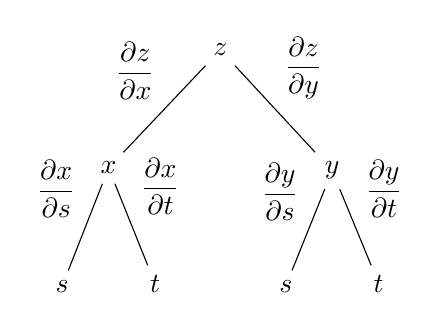
\begin{tikzpicture}[level distance=1.5cm,sibling distance=.8cm, 
		edge from parent path={(\tikzparentnode) -- (\tikzchildnode)}]
		\Tree [.\node {$z$};
		\edge node[auto=right] {$\displaystyle{\frac{\partial z}{\partial x}}$}; 
		[.$x$  
		\edge node[auto=right] {$\displaystyle{\frac{\partial x}{\partial s}}$};  
		[.$s$  ]
		\edge node[auto=left] {$\displaystyle{\frac{\partial x}{\partial t}}$};
		 [.$t$ ]
		]
		\edge node[auto=left] {$\displaystyle{\frac{\partial z}{\partial y}}$};
		[.$y$
		\edge node[auto=right] {$\displaystyle{\frac{\partial y}{\partial s}}$};
		[.$s$ ]
		 \edge node[auto=left] {$\displaystyle{\frac{\partial y}{\partial t}}$};
		 [.$t$ ]
		] ]
		\end{tikzpicture}	
	\end{center}
	We start at the top with the function itself and the branch out from that point. The first set of branches is for the variables in the function. From each of these endpoints we put down a further set of branches that gives the variables that both $ x $ and $ y $ are a function of. We connect each letter with a line and each line represents a partial derivative as shown. Note that the letter in the numerator of the partial derivative is the upper ``node'' of the tree and the letter in the denominator of the partial derivative is the lower ``node'' of the tree. Note that we don't usually put the derivatives in the tree. They are always an assumed part of the tree.
	
	\section{Directional Derivatives}
	
	To this point we've only looked at the two partial derivatives $ f_x(x,y) $ and $ f_y(x,y) $. Recall that these derivatives represent the rate of change of $ f $ as we vary $ x $ (holding $ y $ fixed) and as we vary $ y $ (holding $ x $ fixed) respectively. We now need to discuss how to find the rate of change of $ f $ if we allow both $ x $ and $ y $ to change simultaneously. The problem here is that there are many ways to allow both $ x $ and $ y $ to change. For instance one could be changing faster than the other and then there is also the issue of whether or not each is increasing or decreasing.\\ \\
	The rate of change of $ f(x,y) $ in the direction of the unit vector $ \vec{u} = \langle a,b \rangle $ is called the \textit{directional derivative} and is denoted by $ D_{\vec{u}} f(x,y)$. The definition of the directional derivative is
	\[ D_{\vec{u}} f(x,y) = \lim_{h \to 0} \frac{f(x+ah,y+bh) - f(x,y)}{h} \]
	So, the definition of the directional derivative is very similar to the definition of partial derivatives. However, in practice this can be a very difficult limit to compute so we need an easier way of taking directional derivatives. It's actually fairly simple to derive an equivalent formula for taking directional derivatives. To see how we can do this let's define a new function of a single variable,
	\[ g(z) = f(x_0+az,y_0+bz) \]
	where $ x_0,y_0,a,b $ are fixed numbers. Then by the definition of the derivative for functions of a single variable we have,
	\[ g'(z) = \lim_{h \to 0} \frac{g(z+h) - g(z)}{h} \]
	and the derivative at $ z = 0 $ is given by,
	\[ g'(0) = \lim_{h \to 0} \frac{g(h) - g(0)}{h} \]
	If we now substitute in for $ g(z) $ we get 
	\[ g'(0) = \lim_{h \to 0} \frac{g(h) - g(0)}{h} = \lim_{h \to 0} \frac{f(x_0+ah,y_0+bh) - f(x_0,y_0) }{h} = D_{\vec{u}} f(x_0,y_0) \]
	So it looks like we have the following relationship
	\begin{equation}
		g'(0) = D_{\vec{u}} f(x_0,y_0)
	\end{equation}
	Now let's look at this from another perspective. Let's rewrite $ g(z) $ as follows,
	\[ g(z) = f(x,y) \text{ where } x = x_0+az,\, y = y_0+bz \]
	We can now use the chain rule from the previous section to compute,
	\[ g'(z) = \frac{dg}{dz} = \frac{\partial f}{\partial x} \frac{dx}{dz} + \frac{\partial f}{\partial y} \frac{dy}{dz} = f_x(x,y)a + f_y(x,y)b \]
	So, from the chain rule we get the following relationship.
	\begin{equation}
		g'(z) = f_x(x,y)a + f_y(x,y)b
	\end{equation}
	If we now take $ z = 0 $ we will get that $ x = x_0 $ and $ y = y_0 $ (from how we defined $ x $ and $ y $ above) and plug these into (3.2) we get,
	\begin{equation}
		g'(0) = f_x(x_0,y_0)a + f_y(x_0,y_0)b
	\end{equation}
	Now, simply equate (3.1) and (3.3) to get that,
	\[ D_{\vec{u}} f(x_0,y_0) = g'(0) = f(x_0,y_0)a + f(x_0,y_0)b \]
	If we now go back to allowing $ x $ and $ y $ to be any number we get the following formula for computing directional derivatives.
	\[ D_{\vec{u}} f(x,y) = f_x(x,y)a + f_y(x,y)b \]
	Which is much simpler than the limit definition. Also note that this definition assumed that we were working with functions of two variables. There are similar formulas that can be derived by the same type of argument for functions with more than two variables. For instance, the directional derivative of $ f(x,y,z) $ in the direction of the unit vector $ \vec{u} = \langle a,b,c \rangle $ is given by,
	\[ D_{\vec{u}} f(x,y,z) = f_x(x,y,z)a + f_y(x,y,z)b + f_z(x,y,z)c \]\\
	There is another form of the formula that we used to get the directional derivative that is a little nicer and somewhat more compact.  It is also a much more general formula that will encompass both of the formulas above. Let's start with the second one and notice that we can write it as follows,
	\begin{align*}
		D_{\vec{u}} f(x,y,z) &= f_x(x,y,z)a + f_y(x,y,z)b + f_z(x,y,z)c\\
		&= \langle f_x,f_y,f_z \rangle \cdot \langle a,b,c \rangle		
	\end{align*}
	Now let's give a name and notation to the first vector in the dot product since this vector will show up fairly regularly throughout this course (and in other courses). The \textit{gradient} of $ f $ or \textit{gradient vector} of $ f $ is defined to be,
	\[ \nabla f = \langle f_x,f_y,f_z \rangle   \]
	Or, if we want to use the standard basis vectors the gradient is,
	\[ \nabla f = f_x\uvec{\i} + f_y\uvec{\j} + f_z \uvec{k} \]
	With the definition of the gradient we can now say that the directional derivative is given by,
	\[ D_{\vec{u}} f = \nabla f \cdot \vec{u} \]
	
	
	\chapter{Applications of Partial Derivatives}
	
	In this section we will take a look at a couple of applications of partial derivatives. Most of the applications will be extensions to applications to ordinary derivatives that we saw back in Calculus I. For instance, we will be looking at finding the absolute and relative extrema of a function and we will also be looking at optimization. Both of these subjects were major applications back in Calculus I. They will, however, be a little more work here because we now have more than one variable.
	
	\section{Tangent Planes and Linear Approximations}
	
	The graph of a function $ z = f(x,y) $ is a surface in $ \R^3 $ and we can now start thinking of a  plane that is ``tangent'' to the surface as a point. Let's start out with a point $ (x_0,y_0) $ and let's let $ C_1 $ represent the trace to $ f(x,y) $ for the plane $ y = y_0 $ (i.e. allowing $ x $ to vary with $ y $ held fixed) and we'll let $ C_2 $ represent the trace to $ F(x,y) $ for the plane $ x = x_0 $ (i.e. allowing $ y $ to vary with $ x $ held fixed). Now, we know that $ f_x(x_0,y_0) $ is the slope of the tangent line to the trace $ C_1 $ and $ f_y(x_0,y_0) $ is the slope of the tangent line to the trace $ C_2 $. So, let $ L_1 $ be the tangent line to the trace $ C_2 $ and let $ L_2 $ be the tangent line to the trace $ C_2 $.\\ \\
	The tangent plane will then be the plane that contains the two lines $ L_1 $ and $ L_2 $. Geometrically this plane will serve the same purpose that a tangent line did in Calculus I. A tangent line to a curve was a line that just touched the curve at that point and was ``parallel'' to the curve at the point in question. Well tangent planes to a surface are planes that just touch the surface at the point and are ``parallel'' to the surface at the point. Note that this gives us a point that is on the plane. Since the tangent plane and the surface touch at $ (x_0,y_0) $ the following point will be on both the surface and the plane.
	\[ (x_0,y_0,z_0) = (x_0,y_0,f(x_0,y_0)) \]
	What we need to do now is determine the equation of the tangent plane. We know that the general equation of a plane is given by,
	\[ a(x-x_0) + b(y-y_0) + c(z-z_0) = 0 \]
	where $ (x_0,y_0,z_0) $ is a point that is on the plane, which we know already. Let's rewrite this a little. We'll move the $ x $ terms and $ y $ terms to the other side and divide both sides by $ c $. Doing this gives,
	\[ z - z_0 = -\frac{a}{c}(x-x_0) - \frac{b}{c}(y-y_0) \]
	Now, let's rename the constants to simplify up the notation a little. Let's rename them as follows,
	\[ A = -\frac{a}{c} \qquad B = -\frac{b}{c} \]
	With this renaming the equation of the tangent plane becomes,
	\[ z - z_0 = A(x-x_0) + B(y-y_0) \]
	and we need to determine values for $ A $ and $ B $.  \\ \\
	Let's first think about what happens if we hold $ y $ fixed, i.e. if we assume that $ y = y_0 $. In this case the equation of the tangent plane becomes,
	\[ z - z_0 = A(x-x_0) \]
	This is the equation of a line and this line must be tangent to the surface at $ (x_0,y_0) $ (since it's part of the tangent plane). In addition, this line assumes that $ y = y_0 $ (i.e. fixed) and $ A $ is the slope of this line. But if we think about it this is exactly what the tangent to $ C_1 $ is, a line tangent to the surface at $ (x_0,y_0) $ assuming that $ y = y_0 $. In other words, 
	\[ z - z_0 = A(x-x_0) \]
	is the equation for $ L_1 $ and we know that the slope of $ L_1 $ is given by $ f_x(x_0,y_0) $. Therefore we have the following,
	\[ A = f_x(x_0,y_0) \]
	If we hold $ x $ fixed at $ x = x_0 $ the equation of the tangent plane becomes,
	\[ z - z_0 = B(y-y_0) \]
	However, by a similar argument to the one above we can see that this is nothing more than the equation for $ L_2 $ and that it's slope is $ B $ or $ f_y(x_0,y_0) $. So,
	\[ B = f_y(x_0,y_0) \]
	The equation of the tangent plane to the surface given by $ z = f(x,y) $ at $ (x_0,y_0) $ is then,
	\[ z - z_0 = f_x(x_0,y_0)(x-x_0) + f_y(x_0,y_0)(y-y_0) \]\\
	One nice use of tangent planes is they give us a way to approximate a surface near a point. As long as we are near to the point $ (x_0,y_0) $ then the tangent plane should nearly approximate the function at that point. Because of this we define the linear approximation to be,
	\[ L(x,y) = f(x_0,y_0) + f_x(x_0,y_0)(x-x_0) + f_y(x_0,y_0)(y-y_0) \]
	and as long as we are ``near'' $ (x_0,y_0) $ then we should have that,
	\[ f(x,y) \approx L(x,y) = f(x_0,y_0) + f_x(x_0,y_0)(x-x_0) + f_y(x_0,y_0)(y-y_0) \]
	
	\section{Gradient Vector, Tangent Planes and Normal Lines}
	
	Let's first recall the equation of a plane that contains the point $ (x_0,y_0,z_0) $ with normal vector $ \vec{n} = \langle a,b,c \rangle $ is given by,
	\[ a(x-x_0) + b(y-y_0) + c(z-z_0) = 0 \]
	When we introduced the gradient vector we gave the following fact.\\ \\
	\textbf{Fact}\\
	The gradient vector $ \nabla f(x_0,y_0) $ is orthogonal to the level curve $ f(x,y) = k $ at the point $ (x_0,y_0) $. Likewise, the gradient vector $ \nabla f(x_0,y_0,z_0) $ is orthogonal to the level surface $ f(x,y,z) = k $ at the point $ (x_0,y_0,z_0) $.\\ \\
	Also recall that the gradient vector is,
	\[ \nabla f = \langle f_x,f_y,f_z \rangle \]
	So, the tangent plane to the surface given by $ f(x,y,z) = k $ at $ (x_0,y_0,z_0) $ has the equation,
	\[ f_x(x_0,y_0,z_0)(x-x_0) + f_y(x_0,y_0,z_0)(y-y_0) + f_z(x_0,y_0,z_0)(z-z_0) = 0 \]
	This is a much more general form of the equation of a tangent plane than the one that we derived in the previous section.\\ \\
	Note however, that we can also get the equation from the previous section using this more general formula. To see this let's start with the equation $ z = f(x,y) $ and we want to find the tangent plane to the surface given by $ z = f(,y) $ at the point $ (x_0,y_0,z_0) $ where $ z_0 = f(x_0,y_0) $. In order to use the formula above we need to have all the variables on one side. This is easy enough to do. All we need to do is subtract a $ z $ from both sides to get,
	\[ f(x,y) - z = 0 \]
	Now, if we define a new function 
	\[ F(x,y,z) = f(x,y) - z \]
	we can see that the surface given by $ z = f(x,y) $ is identical to the surface given by $ F(x,y,z) = 0 $ and this new equivalent equation is in the correct form for the equation of the tangent plane that we derived in this section.
	So, the first thing that we need to do is find the gradient vector for $ F $.
	\[ \nabla F = \langle F_x,F_y,F_z \rangle = \langle f_x,f_y,-1 \rangle \]
	The equation of the tangent plane is then,
	\[ f_x(x_0,y_0)(x-x_0) + f_y(x_0,y_0)(y-y_0) - (z-z_0) = 0 \]
	Or, upon solving for $ z $, we get,
	\[ z = f(x_0,y_0) + f_x(x_0,y_0)(x-x_0) + f_y(x_0,y_0)(y-y_0) \]
	which is identical to the equation that we derived in the previous section. We can get another nice piece of information out of the gradient vector as well. We might on occasion want a line that is orthogonal to a surface at a point, sometimes called the \textit{normal line}. This is easy enough to get if we recall that the equation of a line only requires that we have a point and a parallel vector. Since we want a line that is at the point $ (x_0,y_0,z_0) $ we know that this point must also be on the line and we know that $ \nabla f(x_0,y_0,z_0) $ is a vector that is normal to the surface and hence will be parallel to the line.  Therefore the equation of the normal line is,
	\[ \vec{r}(t) = \langle x_0,y_0,z_0) + t\nabla f(x_0,y_0,z_0) \]
	
	\section{Relative Minimums and Maximums}
	
	We are going to be looking at identifying relative minimums and relative maximums. Recall as well that we will often use the word extrema to refer to both minimums and maximums.\\ \\
	\textbf{Definition}
	\begin{enumerate}
		\item A function $ f(x,y) $ has a \textit{relative minimum} at the point $ (a,b	) $ if $ f(x,y) \geq f(a,b) $ for all points $ (x,y) $ in some region around $ (a,b)$.
		\item A function $ f(x,y) $ has a \textit{relative maximum} at the point $ (a,b	) $ if $ f(x,y) \leq f(a,b) $ for all points $ (x,y) $ in some region around $ (a,b)$.
	\end{enumerate}
	Next we need to extend the idea of critical points up to functions of two variables. Recall that a critical point of the function $ f(x) $ was a number $ x = c $ so that either $ f'(c = 0) $ or $ f'(c) $ doesn't exist. We have a similar definition for critical points of functions of two variables.\\ \\
	\textbf{Definition}\\
	The point $ (a,b) $ is a \textit{critical point} of $ f(x,y) $ provided one of the following is true,
	\begin{enumerate}
		\item $ \nabla f(a,b) = \vec{0} $ (this is equivalent to saying that $ f_x(a,b) = 0 $ and $ f_y(a,b) = 0 $).
		\item $ f_x(a,b) $ and/or $ f_y(a,b) $ does not exist.
	\end{enumerate}
	To see the equivalence in the first part let's start off with $ \nabla f = \vec{0} $ and put in the definition of each part.
	\begin{align*}
		\nabla f(a,b) &= \vec{0}\\
		\langle f_x(a,b), f_y(a,b) \rangle &= \langle 0,0 \rangle
	\end{align*}
	The only way that these two vectors can be equal is to have $ f_x(a,b) = 0 $ and $ f_y(a,b) = 0 $. In fact, we will use this definition of the critical point more than the gradient definition since it will be easier to find the critical points if we start with the partial derivative definition. We now have the following fact that, at least partially, relates critical points to relative extrema.\\ \\
	\textbf{Fact}\\
	If the point $ (a,b) $ is a relative extrema of the function $ f(x,y) $ and the first order derivatives of $ f(x,y) $ exist at $ (a,b) $ then $ (a,b) $ is also a critical point of $ f(x,y) $ and in fact we'll have $ \nabla f(a,b) = \vec{0} $.\\ \\
	Note that this does NOT say that all critical points are relative extrema. It only says that relative extrema will be critical points of the function. To see this let's consider the function
	\[ f(x,y) = xy \]
	The two first order partial derivatives are
	\[ f_x = y \qquad f_y = x \]
	The only point that will make both of these derivatives zero at the same time is $ (0,0) $ and so $ (0,00) $ is a critical point for the function. Here is a graph of the function.
	\begin{center}
		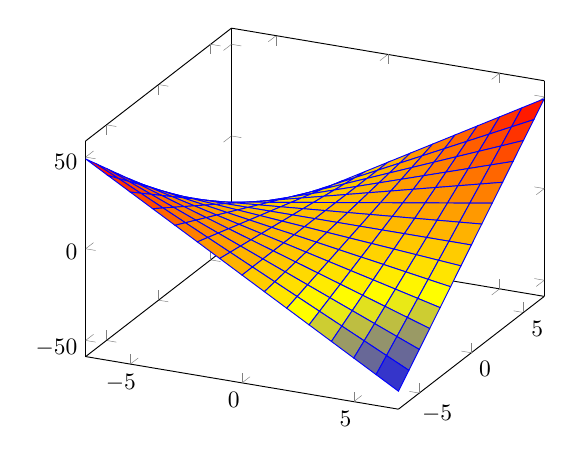
\begin{tikzpicture}[scale=0.85]
			\begin{axis}
			\addplot3
				[surf,faceted color=blue,
				samples=15,
				domain=-7:7,y domain=-7:7]
				{x*y};
			\end{axis}
		\end{tikzpicture}
	\end{center}
	Note that the axes are not in the standard orientation here so that we can see more clearly what is happening at the origin, i.e. at $ (0,0) $. If we start at the origin and move into either of the quadrants where both $ x $ and $ y $ are the same sign the function increases. However, if we start at the origin and move into either of the quadrants where $ x $ and $ y $ have the opposite sign then the function decreases. In other words, no matter what region you take about the origin there will be points larger than $ f(0,0) = 0 $ and points smaller than $ f(0,0) = 0 $. Therefore, there is no way that $ (0,0) $ can be a relative extrema. Critical points that exhibit this kind of behavior are called \textit{saddle points}.\\ \\
	So, once we have all the critical points in hand all we will need to do is test these points to see if they are relative extrema or not. To determine if a critical point is a relative extrema (and in fact to determine if it is a minimum or a maximum) we can use the following fact.\\ \\
	\textbf{Fact}\\
	Suppose that $ (a,b) $ is a critical point of $ f(x,y) $ and that the second order partial derivatives are continuous in some region that contains $ (a,b) $. Next define,
	\[ D(a,b) = f_{xx}(a,b)f_{yy}(a,b) - \left[ f_{xy}(a,b) \right]^2 \]
	We then have the following classifications of the critical point
	\begin{enumerate}
		\item If $ D > 0 $ and $ f_{xx}(a,b) > 0 $ then there is a relative minimum at $ (a,b) $.
		\item If $ D > 0 $ and $ f_{xx}(a,b) < 0 $ then there is a relative maximum at $ (a,b) $.
		\item If $ D < 0 $ then $ (a,b) $ is a saddle point.
		\item If $ D = 0 $ then the point $ (a,b) $ may be a relative minimum, relative maximum or a saddle point.
	\end{enumerate}

	
	\section{Absolute Minimums and Maximums}
	
	In this section we want to optimize a function, that is identify the absolute minimum and/or the absolute maximum of the function, on a given region in $ \R^2 $. Note that when we say we are going to be working on a region in $ \R^2 $ we mean that we're going to be looking at some region in the $ xy $-plane. In order to optimize a function in a region we are going to need to get a couple of definitions out of the way and a fact. Let's first get the definitions out of the way.\\ \\
	\textbf{Definitions}
	\begin{enumerate}
		\item A region in $ \R^2 $ is called \textit{closed} if it includes its boundary. A region is called \textit{open} if it doesn't include any of its boundary points.
		\item A region in $ \R^2 $ is called \textit{bounded} if it can be completely contained in a disk. In other words, a region will be bounded if it is finite.
	\end{enumerate}
	Let's think a little more about the definition of closed. We said a region is closed if it includes its boundary. Just what does this mean? Let's think of a rectangle. Below are two definitions of a rectangle, one is closed and the other is open.
	
	\begin{center}
		\begin{tabular}{cc}
			Open & Closed\\
			$ -5 < x < 3 $ & $ -5 \leq x \leq 3 $\\
			$ 1 < y < 6 $ & $ 1 \leq y \leq 6 $
		\end{tabular}
	\end{center}
	In this first case we don't allow the ranges to include the endpoints (i.e. we aren't including the edges of the rectangle) and so we aren't allowing the region to include any points on the edge of the rectangle. In other words, we aren't allowing the region to include its boundary and so it's open. In the second case we are allowing the region to contain points on the edges and so will contain its entire boundary and hence will be closed. This is an important idea because of the following fact.\\ \\
	\textbf{Extreme Value Theorem}\\
	If $ f(x,y) $ is continuous in some closed, bounded set $ D $ in $ \R^2 $ then there are points in $ D $, $ (x_1,y_1) $ and $ (x_2,y_2) $ so that $ f(x_1,y_1) $ is the absolute maximum and $ f(x_2,y_2) $ is the absolute minimum of the function in $ D $.\\ \\
	Note that this theorem does NOT tell us where the absolute minimum or absolute maximum will occur. It only tells us that they will exist. Note as well that the absolute minimum and/or absolute maximum may occur in the interior of the region or it may occur on the boundary of the region.\\ \\
	The basic process for finding absolute maximums is pretty much identical to the process that we used in Calculus I when we looked at finding absolute extrema of functions of single variables. There will however, be some procedural changes to account for the fact that we now are dealing with functions of two variables. Here is the process.\\ \\
	\textbf{Finding Absolute Extrema}
	\begin{enumerate}
		\item Find all the critical points of the function that lie in the region $ D $ and determine the function value at each of these points.
		\item Find all extrema of the function on the boundary. This usually involves the Calculus I approach for this work.
		\item The largest and smallest values found in the first two steps are the absolute minimum and the absolute maximum of the function.
	\end{enumerate}
	The main difference between this process and the process that we used in Calculus I is that the ``boundary'' in Calculus I was just two points and so there really wasn't a lot to do in the second step. For these problems the majority of the work is often in the second step as we will often end up doing a Calculus I absolute extrema problem one or more times.
	
	\section{Lagrange Multipliers}
	
	In this section we are going to take a look at another way of optimizing a function subject to given constraint(s). The constraint(s) may be the equation(s) that describe the boundary of a region although in this section we won't concentrate on those types of problems since this method just requires a general constraint and doesn't really care where the constraint came from.\\ \\
	We want to optimize (i.e. find the minimum and maximum value of) a function, $ f(x,y,z) $, subject to the constraint $ g(x,y,z) = k $. Again, the constraint may be the equation that describes the boundary of a region or it may not be. The process is actually fairly simple, although the work can still be a little overwhelming at times.\\ \\
	\textbf{Method of Lagrange Multipliers}
	\begin{enumerate}
		\item Solve the following system of equations
		\begin{align*}
			\nabla f(x,y,z) &= \lambda \,  \nabla g(x,y,z)\\
			g(x,y,z) &= k
		\end{align*}
		\item Plug in all solutions, $ (x,y,z) $, from the first step into $ f(x,y,z) $ and identify the minimum and maximum values, provided they exist.
	\end{enumerate}
	The constant, $ \lambda $, is called the \textit{Lagrange Multiplier}.\\ \\
	Notice that the system of equations actually has four equations, we just wrote the system in a simpler form. To see this let's take the first equation and put in the definition of the gradient vector to see what we get.
	\begin{align*}
		\langle f_x,f_y,f_z \rangle &= \lambda \langle g_x,g_y,g_z \rangle\\
		&= \langle \lambda\,g_x,\lambda\,g_y,\lambda\,g_z \rangle 
	\end{align*}
	In order for these two vectors to be equal the individual components must also be equal. So, we actually have three equations here.
	\[ f_x = \lambda \, g_x \qquad f_y = \lambda \, g_y \qquad f_z = \lambda \, g_z \]
	These three equations along with the constraint, $ g(x,y,z) = k $, give four equations with four unknowns $ x $, $ y $, $ z $, and $ \lambda $.\\ \\
	Naturally, we can extend this to multiple constraints. Suppose we want to optimize $ f(x,y,z) $ subject to the constraints $ g(x,y,z) = c $ and $ h(x,y,z) = k $. The system that we need to solve in this case is,
	\begin{align*}
		\nabla f(x,y,z) &= \lambda \, \nabla g(x,y,z) + \mu \, \nabla h(x,y,z)\\
		g(x,y,z) &= c\\
		h(x,y,z) &= k
	\end{align*}
	
	\chapter{Multiple Integrals}
	
	In Calculus I we moved on to the subject of integrals once we had finished the discussion of derivatives. The same is true in this course. Now that we have finished our discussion of derivatives of functions of more than one variable we need to move on to integrals of functions of two or three variables.\\ \\
	Most of the derivatives topics extended somewhat naturally from their Calculus I counterparts and that will be the same here. However, because we are now involving functions of two or three variables there will be some differences as well.  here will be new notation and some new issues that simply don't arise when dealing with functions of a single variable.  
	
	\section{Double Integrals}
	
	Before starting on double integrals let's do a quick review of the definition of a definite integrals for functions of single variables. First, when working with the integral,
	\[ \int\limits_a^b f(x)\,dx \]
	we think of $ x $'s as coming from the interval $ a \leq x \leq b $. For these integrals we can say that we are integrating over the interval $ a \leq x \leq b $. Note that this does assume that $ a<b $, however, if we have $ b>a $ then we can just use the interval $ b \leq x \leq a $.\\ \\
	Now, when we derived the definition of the definite integral we first thought of this as an area problem. We first asked what the area under the curve was and to do this we broke up the interval $ a \leq x \leq b $ into $ n $ subintervals of width $ \Delta x $ and choose a point,  $ x_i^* $, from each interval. Each of the rectangles has height of $ f(x_i^*) $  and we could then use the area of each of these rectangles to approximate the area as follows.
	\[ A \approx f(x_1^*) \Delta x + f(x_2^*) \Delta x + \ldots + f(x_i^*) \Delta x + \ldots + f(x_n^*) \Delta x  \]
	To get the exact area we then took the limit as $ n $ goes to infinity and this was also the definition of the definite integral.
	\[ \int\limits_a^b f(x)\,dx = \lim_{n \to \infty} \sum_{i=1}^{\infty} f(x_i^*) \Delta x \]
	In this section we want to integrate a function of two variables, $ f(x,y) $. With functions of one variable we integrated over an interval (i.e. a one-dimensional space) and so it makes some sense then that when integrating a function of two variables we will integrate over a region of $ \R^2 $.\\ \\
	We will start out by assuming that the region in $ \R^2 $ is a rectangle which we will denote as follows,
	\[ R = [ a,b ] \times [ c,d ] \]
	This means that the ranges for $ x $ and $ y $ are $ a \leq x \leq b $ and $ c \leq y \leq d $. Also, we will initially assume that $ f(x,y) > 0 $ although this doesn't really have to be the case. Let's start out with the graph of the surface $ S $ given by graphing $ f(x,y) $ over the rectangle $ R $.
	
	\begin{center}
		\tdplotsetmaincoords{70}{120}
		\begin{tikzpicture}[tdplot_main_coords]
		
		% Axis
		\draw[->] (0,0,0) -- (4,0,0) node[left] {$x$};
		\draw[->] (0,0,0) -- (0,4,0) node[right] {$y$};
		\draw[->] (0,0,0) -- (0,0,3) node[above] {$z$};
		
		% Rectangle
		\draw[dashed] (1,0,0) -- (1,1,0);
		\draw[dashed] (2.5,0,0) -- (2.5,1,0);
		\draw[dashed] (0,1,0) -- (1,1,0);
		\draw[dashed] (0,2.5,0) -- (1,2.5,0);
		\draw (1,1,0) -- (2.5,1,0) -- (2.5,2.5,0) -- (1,2.5,0) -- (1,2.5,0) -- (1,1,0);
		\fill[cyan!50,opacity=0.6] (1,1,0) -- (2.5,1,0) -- (2.5,2.5,0) -- (1,2.5,0) -- (1,2.5,0) -- (1,1,0);
		
		% Nodes
		\draw (1,0,0) node[left=1mm] {$a$};
		\draw (2.5,0,0) node[left=1mm] {$b$};
		\draw (0,1,0) node[above] {$c$};
		\draw (0,2.5,0) node[above=] {$d$};
		\draw (2.5,2.5,0) node[below=1mm] {$R$};
		\draw (2,2,2.5) node[above] {$S$};
		
		% Lines to Surface
		\draw[dashed] (1,1,0) -- (1,1,2);
		\draw[dashed] (2.5,1,0) -- (2.5,1,1.5);
		\draw[dashed] (2.5,2.5,0) -- (2.5,2.5,2);
		\draw[dashed] (1,2.5,0) -- (1,2.5,2.5);
		\draw (1,1,2) to[bend left] (2.5,1,1.5);
		\draw (2.5,1,1.5) to[bend right] (2.5,2.5,2);
		\draw (2.5,2.5,2) to[bend right] (1,2.5,2.5);
		\draw (1,2.5,2.5) to[bend left] (1,1,2); 
		\fill[green!50,opacity=0.6] (1,1,2) to[bend left] (2.5,1,1.5) -- (2.5,1,1.5) to[bend right] (2.5,2.5,2) -- (2.5,2.5,2) to[bend right] (1,2.5,2.5) -- (1,2.5,2.5) to[bend left] (1,1,2);
		\end{tikzpicture}
	\end{center}
	Now, just like with functions of one variable let's not worry about integrals quite yet. Let's first ask what the volume of the region under $ S $ (and above the $ xy $-plane of course) is.\\ \\
	We will first approximate the volume much as we approximated the area above. We will first divide up $ a \leq x \leq b $ into $ n $ subintervals and divide up $ c \leq y \leq d $ into $ m $ subintervals.  This will divide up $ R $ into a series of smaller rectangles and from each of these we will choose a point $ (x_i^*,y_j^*) $. Here is a sketch of this set up. 
	\begin{center}
		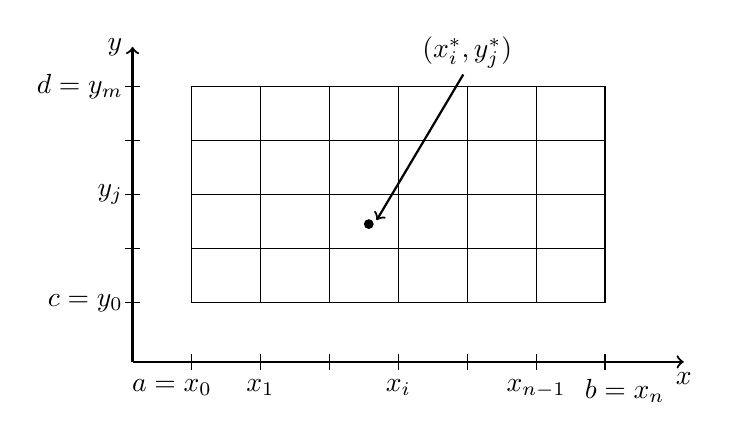
\begin{tikzpicture}
			% Axis
			\draw[thick,->] (0,0) -- (7,0) node[below] {$x$};
			\draw[thick,->] (0,0) -- (0,4) node[left] {$y$};
			
			% Rectangle
			\draw (0.75,0.75) -- (6,0.75);
			\draw (0.75,0.75) -- (0.75,3.5);
			\draw (6,0.75) -- (6,3.5);
			\draw (0.75,3.5) -- (6,3.5);
			
			% Grid
			% x
			\draw (0.75,0.75) -- (0.75,3.5);
			\draw (1.625,0.75) -- (1.625,3.5);
			\draw (2.5,0.75) -- (2.5,3.5);
			\draw (3.375,0.75) -- (3.375,3.5);
			\draw (4.25,0.75) -- (4.25,3.5);
			\draw (5.125,0.75) -- (5.125,3.5);
			\draw (6,0.75) -- (6,3.5);
			% y
			\draw (0.75,1.4375) -- (6,1.4375);
			\draw (0.75,2.125) -- (6,2.125);
			\draw (0.75,2.8125) -- (6,2.8125);
						
			% Ticks
			% x
			\draw (0.75,-0.1) -- (0.75,0.1);
			\draw (1.625,-0.1) -- (1.625,0.1);
			\draw (2.5,-0.1) -- (2.5,0.1);
			\draw (3.375,-0.1) -- (3.375,0.1);
			\draw (4.25,-0.1) -- (4.25,0.1);
			\draw (5.125,-0.1) -- (5.125,0.1);
			\draw (6,-0.1) -- (6,0.1);
			% y
			\draw (-0.1,0.75) -- (0.1,0.75);
			\draw (-0.1,1.4375) -- (0.1,1.4375);
			\draw (-0.1,2.125) -- (0.1,2.125);
			\draw (-0.1,2.8125) -- (0.1,2.8125);
			\draw (-0.1,3.5) -- (0.1,3.5);
			
			% nodes
			% x 
			\draw (0.5,0) node[below=1mm] {$a = x_0$};
			\draw(1.625,0) node[below=1mm] {$x_1$};	
			\draw (3.375,0) node[below=1mm] {$x_i$};
			\draw (5.125,0) node[below=1mm] {$x_{n-1}$};
			\draw (6.25,0) node[below=1mm] {$b = x_n$};
			% y
			\draw (0,0.75) node[left] {$c=y_0$};
			\draw (0,2.125) node[left] {$y_j$};
			\draw (0,3.5) node[left] {$d = y_m$};
			
			% center thing
			\node[fill,circle,inner sep=1.25pt] at (3,1.75) {};
			\draw (4.25,3.6) node[above] {$(x_i^*,y_j^*)$};
			\draw[<-,thick] (3.1,1.8) -- (4.2,3.65);
			
		\end{tikzpicture}
	\end{center}
	Now, over each of these smaller rectangles we will construct a box whose height is given by $ f(x_i^*,y_j^*) $. Each of the rectangles has a base area of $ \Delta A $ and a height of $ f(x_i^*,y_j^*) $ so the volume of each of these boxes is $ f(x_i^*,y_j^*) \Delta A $. The volume under the surface $ S $ is then approximately,
	\[ V \approx \sum_{i=1}^{n} \sum_{j=1}^{m} f(x_i^*,y_j^*) \Delta A \]
	We will have a double sum since we will need to add up volumes in both the $ x $ and $ y $ directions. To get a better estimation of the volume we will take $ n $ and $ m $ larger and larger and to get the exact volume we will need to take the limit as both $ n $ and $ m $ go to infinity. In other words,
	\[ V = \lim_{n,m \to \infty} \sum_{i=1}^{n} \sum_{j=1}^{m} f(x_i^*,y_j^*) \Delta A \]
	Now, this should look familiar. This looks a lot like the definition of the integral of a function of single variable. In fact this is also the definition of a double integral, or more exactly an integral of a function of two variables over a rectangle.\\ \\
	Here is the official definition of a double integral of a function of two variables over a rectangular region $ R $ as well as the notation that we'll use for it.
	\[ \iint\limits_R f(x,y)\,dA = \lim_{n,m \to \infty} \sum_{i=1}^{n} \sum_{j=1}^{m} f(x_i^*,y_j^*) \Delta A \]
	Note that one interpretation of the double integral of $ f(x,y) $ over the rectangle $ R $ is the volume under the function $ f(x,y) $ (and above the $ xy $-plane).  Or,
	\[ \text{Volume} = \iint\limits_R f(x,y)\,dA \]
	
	\section{Iterated Integrals}
	
	The following theorem tells us how to compute a double integral over a rectangle.\\ \\
	\textbf{Fubini's Theorem}\\
	If $ f(x,y) $ is continuous on $ R = [a,b] \times [c,d] $ then,
	\[ \iint\limits_R f(x,y)\,dA = \int\limits_a^b \int\limits_c^d f(x,y)\,dy\,dx = \int\limits_c^d \int\limits_a^b f(x,y)\,dx\,dy \]
	These integrals are called \textit{iterated integrals}\\ \\
	Note that there are in fact two ways of computing a double integral and also notice that the inner differential matches up with the limits on the inner integral and similarly for the outer differential and limits.  In other words, if the inner differential is $ dy $ then the limits on the inner integral must be $ y $ limits of integration and if the outer differential is $ dy $ then the limits on the outer integral must be $ y $ limits of integration.\\ \\
	Now, on some level this is just notation and doesn't really tell us how to compute the double integral. Let's just take the first possibility above and change the notation a little.
	\[ \iint\limits_R f(x,y)\,dA = \int\limits_a^b \left[ \int\limits_c^d f(x,y)\,dy \right] dx  \]
	We will compute the double integral by first computing 
	\[ \int\limits_c^d f(x,y)\,dy \]
	and we compute this by holding $ x $ constant and integrating with respect to $ y $ as if this were a single integral. This will give a function involving only $ x $'s which we can in turn integrate.\\ \\
	We've done a similar process with partial derivatives. To take the derivative of a function with respect to $ y $ we treated the $ x $'s as constants and differentiated with respect to $ y $ as if it was a function of a single variable. Double integrals work in the same manner. We think of all the $ x $'s as constants and integrate with respect to $ y $ or we think of all $ y $'s as constants and integrate with respect to $ x $.\\ \\
	The next topic of this section is a quick fact that can be used to make some iterated integrals somewhat easier to compute on occasion.\\ \\
	\textbf{Fact}\\
	If $ f(x,y) = g(x)\,h(y) $ and we are integrating over the rectangle $ R = [a,b] \times [c,d] $ then
	\[ \iint\limits_R f(x,y)\,dA = \iint\limits_R g(x)\,h(y)\,dA = \left( \int\limits_a^b g(x)\,dx \right) \left( \int\limits_c^d h(y)\,dy \right) \] 
	So, if we can break up the function into a function only of $ x $ times a function of $ y $ then we can do the two integrals individually and multiply them together.
	
	\section{Double Integrals Over General Regions}
	
	In the previous section we looked at double integrals over rectangular regions. The problem with this is that most of the regions are not rectangular so we need to now look at the following double integral,
	\[ \iint\limits_D f(x,y)\,dA \]
	where $ D $ is any region.\\ \\
	There are two types of regions that we need to look at. Here is a sketch of both of them.
	
	\begin{center}
		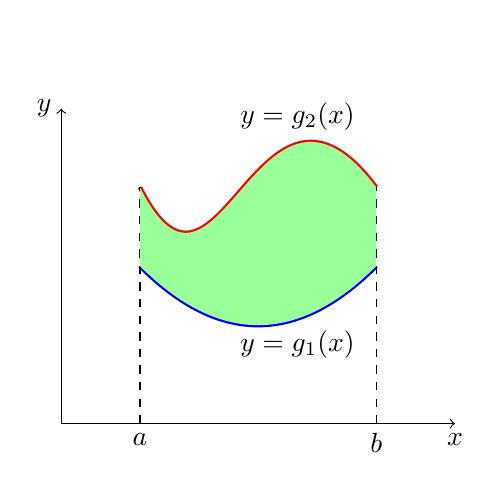
\begin{tikzpicture}
			% Axis
			\draw[->] (0,-1) -- (5,-1) node[below] {$x$};
			\draw[->] (0,-1) -- (0,3) node[left] {$y$};
			
			% Curves
			\draw[ultra thick,draw=red] (1,2) .. controls (2,0) and (2.5,4) .. (4,2);
			\draw[ultra thick,draw=blue] (1,1) .. controls (2,0) and (3,0) .. (4,1);
			\draw[dashed] (1,-1) -- (1,2);
			\draw[dashed] (4,-1) -- (4,2);
			
			% Area
			\path[fill=green!40] (1,1) -- (1,2) -- (1,2) .. controls (2,0) and (2.5,4) .. (4,2) -- (4,1) -- (4,1) -- (1,1) .. controls (2,0) and (3,0) .. (4,1);
			
			% Nodes
			\draw(1,-1) node[below] {$a$};
			\draw(4,-1) node[below] {$b$};
			\draw (3,0) node {$y=g_1(x)$};
			\draw (3,2) node[above=6mm] {$y=g_2(x)$};
		\end{tikzpicture}
		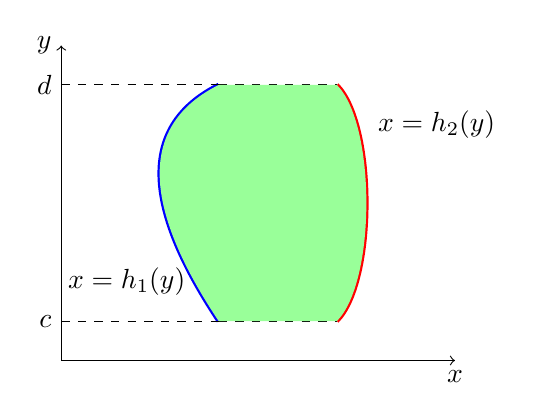
\begin{tikzpicture}
			% Axis
			\draw[->] (-1,-1) -- (4,-1) node[below] {$x$};
			\draw[->] (-1,-1) -- (-1,3) node[left] {$y$};
			
			% Curves
			\draw[ultra thick,draw=blue] (1,2.5) .. controls(0,2) and (0,1) .. (1,-0.5);
			\draw[ultra thick,draw=red] (2.5,2.5) .. controls(3,2) and (3,0) .. (2.5,-0.5);
			\draw[dashed] (1,-0.5) -- (2.5,-0.5);
			\draw[dashed] (1,2.5) -- (2.5,2.5);
			
			% Area
			\path[fill=green!40] (2.5,2.5) .. controls(3,2) and (3,0) .. (2.5,-0.5) -- (1,2.5) .. controls(0,2) and (0,1) .. (1,-0.5) -- (1,-0.5) -- (2.5,-0.5) -- (1,2.5) -- (2.5,2.5);
			
			% Nodes
			\draw[dashed] (-1,-0.5) -- (1,-0.5);
			\draw[dashed] (-1,2.5) -- (1,2.5);
			\draw (-1,-0.5) node[left] {$c$};
			\draw (-1,2.5) node[left] {$d$};
			\draw (0.7,0) node[left] {$x=h_1(y)$};
			\draw (2.7,2) node[right=2mm] {$x=h_2(y)$};
		\end{tikzpicture}
	\end{center}
	We will often use set builder notation to describe these regions. Here is the definition for the region in Case I
	\[ D = \{ (x,y) \, \lvert \, a \leq x \leq b, g_1(x) \leq y \leq g_2(x) \} \]
	and here is the definition for the region in Case II
	\[ D = \{ (x,y) \, \lvert \, h_1(y) \leq x \leq h_2(y), c \leq y \leq d \} \]
	The double integral for both of these cases are defined in terms of iterated integrals as follows.\\ \\
	In Case I where $ D = \{ (x,y) \, \lvert \, a \leq x \leq b, g_1(x) \leq y \leq g_2(x) \} $ the integral is defined to be,
	\[ \iint\limits_D f(x,y)\,dA = \int\limits_a^b \int\limits_{g_1(x)}^{g_2(x)} f(x,y)\,dy\,dx \]
	In Case 2 where $ D = \{ (x,y) \, \lvert \, h_1(y) \leq x \leq h_2(y), c \leq y \leq d \} $ the integral is defined to be,
	\[ \iint\limits_D f(x,y)\,dA = \int\limits_c^d \int\limits_{h_1(y)}^{h_2(y)} f(x,y)\,dx\,dy \]
	Here are some properties of the double integral. Note that all three of these properties are really just extensions of properties of single integrals that have been extended to double integrals.\\ \\
	\textbf{Properties}
	\begin{enumerate}
		\item $ \displaystyle{\iint\limits_D f(x,y) + g(x,y)\,dA = \iint\limits_D f(x,y)\,dA + \iint\limits_D g(x,y)\,dA} $
		\item $ \displaystyle{\iint_D cf(x,y)\,dA = c\iint_D f(x,y)\,dA} $, where $ c $ is any constant.
		\item If the region $ D $ can be split into two separate regions $ D_1 $ and $ D_2 $ then the integral can be written as
		\[ \iint\limits_D f(x,y)\,dA = \iint\limits_{D_1} f(x,y)\,dA + \iint\limits_{D_2} f(x,y)\,dA \]
	\end{enumerate}
	The final topic of this section is two geometric interpretations of a double integral. The first interpretation is an extension of the idea that we used to develop the idea of a double integral in the first section of this chapter. We did this by looking at the volume of the solid that was below the surface of the function $ z = f(x,y) $ and over the rectangle $ R $ in the $ xy $-plane. This idea can be extended to more general regions.\\ \\
	The volume of the solid that lies below the surface given by $ z = f(x,y) $ and above the region $ D $ in the $ xy $-plane is given by,
	\[ V = \iint\limits_D f(x,y)\,dA \]
	The second geometric interpretation of a double integral is the following.
	\[ \text{Area of } D = \iint\limits_D dA \]
	This is easy to see why this is true in general.  Let’s suppose that we want to find the area of the region shown below.
	\begin{center}
		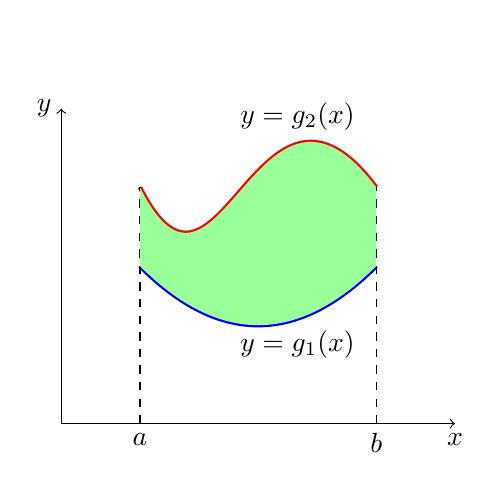
\begin{tikzpicture}
		% Axis
		\draw[->] (0,-1) -- (5,-1) node[below] {$x$};
		\draw[->] (0,-1) -- (0,3) node[left] {$y$};
		
		% Curves
		\draw[ultra thick,draw=red] (1,2) .. controls (2,0) and (2.5,4) .. (4,2);
		\draw[ultra thick,draw=blue] (1,1) .. controls (2,0) and (3,0) .. (4,1);
		\draw[dashed] (1,-1) -- (1,2);
		\draw[dashed] (4,-1) -- (4,2);
		
		% Area
		\path[fill=green!40] (1,1) -- (1,2) -- (1,2) .. controls (2,0) and (2.5,4) .. (4,2) -- (4,1) -- (4,1) -- (1,1) .. controls (2,0) and (3,0) .. (4,1);
		
		% Nodes
		\draw(1,-1) node[below] {$a$};
		\draw(4,-1) node[below] {$b$};
		\draw (3,0) node {$y=g_1(x)$};
		\draw (3,2) node[above=6mm] {$y=g_2(x)$};
		\end{tikzpicture}
	\end{center}
	From Calculus I we know that this area can be found by the integral,
	\[ A = \int\limits_a^b g_2(x) - g_1(x)\,dx \]
	Or in terms of a double integral we have,
	\begin{align*}
		\text{Area of } D &= \iint\limits_D dA\\
		&= \int\limits_a^b \int\limits_{g_1(x)}^{g_2(x)} dy\,dx\\
		&= \int\limits_a^b y \, \Big|_{g_1(x)}^{g_2(x)}\,dx\\
		&= \int\limits_a^b g_2(x) - g_1(x)\,dx
	\end{align*}
	This is exactly the same formula we had in Calculus I.
	
	\section{Double Integrals in Polar Coordinates}
	
	To this point we've seen quite a few double integrals. However, in every case we've seen to this point the region $ D $ could be easily described in terms of simple functions in Cartesian coordinates. In this section we want to look at some regions that are much easier to describe in terms of polar coordinates. For instance, we might have a region that is a disk, ring, or a portion of a disk or ring. In these cases using Cartesian coordinates could be somewhat cumbersome. For instance let's suppose we wanted to do the following integral,
	\[ \iint\limits_D f(x,y)\,dA,\,\, D \text{ is the disk of radius } 2 \]
	To this we would have to determine a set of inequalities for x and y that describe this region.  These would be, 
	\begin{align*}
		-2 &\leq x \leq 2\\
		-\sqrt{4 - x^2} &\leq y \leq \sqrt{4 - x^2}
	\end{align*}
	With these limits the integral would become,
	\[ \iint\limits_D f(x,y)\,dA = \int\limits_{-2}^{2} \int\limits_{-\sqrt{4 - x^2}}^{\sqrt{4 - x^2}} f(x,y)\,dy\,dx \]
	Due to the limits on the inner integral this is liable to be an unpleasant integral to compute.\\ \\
	However, a disk of radius 2 can be defined in polar coordinates by the following inequalities,
	\begin{align*}
		& 0 \leq r \leq 2\\
		& 0 \leq \theta \leq 2\pi
	\end{align*}
	These are very simple limits and, in fact, are constant limits of integration which almost always makes integrals somewhat easier.\\ \\
	So, if we could convert our double integral formula into one involving polar coordinates we would be in pretty good shape. The problem is that we can't just convert the $ dx $ and the $ dy $ into a $ dr $ and a $ d\theta $.  In computing double integrals to this point we have been using the fact that $ dA = dx\,dy $ and this really does require Cartesian coordinates to use. Once we've moved into polar coordinates $ dA \neq dr\,d\theta $ and so we're going to need to determine just what $ dA $ is under polar coordinates.\\ \\
	So, let's step back a little bit and start off with a general region in terms of polar coordinates and see what we can do with that. Here is a sketch of some region using polar coordinates.
	\begin{center}
		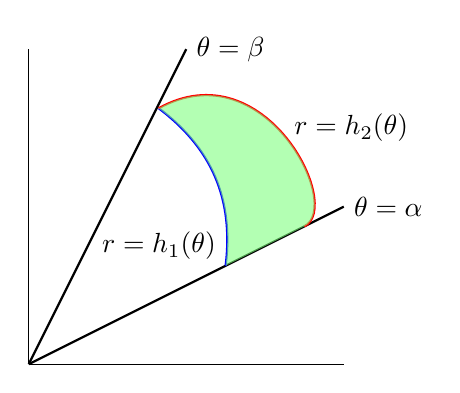
\begin{tikzpicture}
			\draw (0,0) -- (4,0);
			\draw (0,0) -- (0,4);
			
			% Angle parameters
			\draw[thick] (0,0) -- (2,4) node[right] {$\theta = \beta$};
			\draw[thick] (0,0) -- (4,2) node[right] {$\theta = \alpha$};
			
			% Curves
			\draw[thick,draw=blue] (1.65,3.25) to[bend left] (2.5,1.25);
			\draw[thick,draw=red] (1.65,3.25) .. controls(3,4) and (4,2) .. (3.5,1.75);
			
			% Area
			\fill[green!50,opacity=0.6] (1.65,3.25) to[bend left] (2.5,1.25) -- (2.5,1.25) -- (3.5,1.75) -- (1.65,3.25) .. controls(3,4) and (4,2) .. (3.5,1.75);
			
			% Nodes
			\draw (2.5,1.5) node[left] {$r = h_1(\theta)$};
			\draw (3.25,3) node[right] {$r = h_2(\theta)$};
			
		\end{tikzpicture}
	\end{center}
	So, our general region will be defined by inequalities,
	\begin{align*}
		\alpha &\leq \theta \leq \beta\\
		h_1(\theta) &\leq r \leq h_2(\theta)
	\end{align*}
	Now, to find $ dA $ let's redo the figure above as follows,
	\begin{center}
		\includegraphics[scale=0.5]{polar.png}
	\end{center}
	As shown, we'll break up the region into a mesh of radial lines and arcs. Now, if we pull one of the pieces of the mesh out as shown we have something that is almost, but not quite a rectangle. The area of this piece is $ \Delta A $. The two sides of this piece both have length $ \Delta r = r_0 - r_i $ where $ r_0 $ is the radius of the outer arc and $ r_i $ is the radius of the inner arc. Basic geometry then tells us that the length of the inner edge is $ r_i \Delta \theta $ while the length of the out edge is $ r_0 \Delta \theta $ where $ \Delta \theta $ is the angle between the two radial lines that form the sides of this piece.\\ \\
	Now, let's assume that we've taken the mesh so small that we can assume that $ r_i \approx r_0 = r $ and with this assumption we can also assume that our piece is close enough to a rectangle that we can also then assume that,
	\[ \Delta A \approx r\Delta \theta \Delta r \]
	Also, if we assume that the mesh is small enough then we can also assume that,
	\[ dA \approx \Delta A \qquad d\theta \approx \Delta \theta \qquad dr \approx \Delta r \]
	With these assumptions we then get $ dA \approx r\,dr\,d\theta $.\\ \\
	In order to arrive at this we had to make the assumption that the mesh was very small. This is not an unreasonable assumption. Recall that the definition of a double integral is in terms of two limits and as limits go to infinity the mesh size of the region will get smaller and smaller. In fact, as the mesh size gets smaller and smaller the formula above becomes more and more accurate and so we can say that,
	\[ dA = r\,dr\,d\theta \]
	Now, if we're going to be converting an integral in Cartesian coordinates into an integral in polar coordinates we are going to have to make sure that we've also converted all the $ x $'s and $ y $'s into polar coordinates as well. To do this we'll need to remember the following conversion formulas,
	\[ x = r\cos\theta \qquad y = r\sin\theta \qquad r^2 = x^2 + y^2 \]
	Putting this all together we have,
	\[ \iint\limits_D f(x,y)\,dA = \int\limits_{\alpha}^{\beta} \int\limits_{h_1(\theta)}^{h_2(\theta)} f(r\cos\theta, r\sin\theta)\,r\,dr\,d\theta \]
	It is important to not forget the added $ r $ and don't forget to convert the Cartesian coordinates in the function over to polar coordinates.
	
	\section{Triple Integrals}
	
	Now that we know how to integrate over a two-dimensional region we need to move on to integrating over a three-dimensional region. We used a double integral to integrate over a two-dimensional region and so it shouldn't be too surprising that we'll use a triple integral to integrate over a three dimensional region. The notation for the general triple integrals is,
	\[ \iiint\limits_E f(x,y,z)\,dV \]
	Let's start simple by integrating over the box,
	\[ B = [a,b] \times [c,d] \times [u,v] \]
	Note that when using this notation we list the $ x $'s first, the $ y $'s second and the $ z $'s third.\\ \\
	The triple integral in this case is,
	\[ \iiint\limits_E f(x,y,z)\,dV = \int\limits_u^v \int\limits_c^d \int\limits_a^b f(x,y,z)\,dx\,dy\,dz \]
	Note that we integrated with respect to $ x $ first, then $ y $, and finally $ z $ here, but in fact there is no reason to the integrals in this order. There are 6 different possible orders to do the integral in and which order you do the integral in will depend upon the function and the order that you feel will be the easiest. We will get the same answer regardless of the order however.\\ \\
	Before moving on to more general regions let's get a nice geometric interpretation about the triple integral out of the way so we can use it in some of the examples to follow.\\ \\
	\textbf{Fact}\\
	The volume of the three-dimensional region $ E $ is given by the integral,
	\[ V = \iiint\limits_E dV \]
	Let's now move on the more general three-dimensional regions. We have three different possibilities for a general region. Here is a sketch of the first possibility.
	\begin{center}
		\includegraphics[scale=0.6]{trip1.png}
	\end{center}
	In this case we define the region $ E $ as follows,
	\[ E = \{ (x,y,z) \, \lvert \, (x,y) \in D, u_1(x,y) \leq z \leq u_2(x,y) \} \]
	In this case we will evaluate the triple integral as follows,
	\[ \iiint\limits_E f(x,y,z)\,dV = \iint\limits_D \left[ \int\limits_{u_1(x,y)}^{u_2(x,y)} f(x,y,z)\,dz \right]dA \]
	where the double integral can be evaluated in any of the methods that we saw in the previous couple of sections. In other words, we can integrate first with respect to $ x $, we can integrate first with respect to $ y $, or we can use polar coordinates as needed. \\ \\
	Let's now move onto the second possible three-dimensional region we may run into for triple integrals. Here is a sketch of this region.
	\begin{center}
		\includegraphics[scale=0.6]{trip2.png}
	\end{center}
	For this possibility we define the region $ E $ as follows,
	\[ E = \{ (x,y,z) \, \lvert \, (y,z) \in D, u_1(y,z) \leq x \leq u_2(y,z) \} \]
	So, the region $ D $ will be a region in the $ yz $-plane. Here is how we will evaluate these integrals.
	\[ \iiint\limits_E f(x,y,z)\,dV = \iint\limits_D \left[ \int\limits_{u_1(y,z)}^{u_2(y,z)} f(x,y,z)\,dx \right]dA \]
	As with the first possibility we will have two options for doing the double integral in the $ yz $-plane as well as the option of using polar coordinates if needed.\\ \\
	We now need to look at the third (and final) possible three-dimensional region we may run into for triple integrals. Here is a sketch of this region.
	\begin{center}
		\includegraphics[scale=0.6]{trip3.png}
	\end{center}
	In this final case $ E $ is defined as,
	\[ E = \{ (x,y,z) \, \lvert \, (x,z) \in D, u_1(x,z) \leq y \leq u_2(x,z) \} \]
	and here the region $ D $ will be a region in the $ xz $-plane. Here is how we will evaluate these integrals.
	\[ \iiint\limits_E f(x,y,z)\,dV = \iint\limits_D \left[ \int\limits_{u_1(x,z)}^{u_2(x,z)} f(x,y,z)\,dy \right]dA \]
	where we will can use either of the two possible orders for integrating $ D $ in the $ xz $-plane or we can use polar coordinates if needed.

	\section{Triple Integrals in Cylindrical Coordinates}

	In this section we want do take a look at triple integrals done completely in Cylindrical Coordinates. Recall that cylindrical coordinates are really nothing more than an extension of polar coordinates into three dimensions. The following are the conversion formulas for cylindrical coordinates.
	\[ x = r\cos\theta \qquad y = r\sin\theta \qquad z = z \]
	In order to do the integral in cylindrical coordinates we will need to know what $ dV $ will become in terms of cylindrical coordinates. We will be able to show in the Change of Variables section of this chapter that,
	\[ dV = r\,dz\,dr\,d\theta \]
	The region, $ E $, over which we are integrating becomes,
	\begin{align*}
		E &= \{ (x,y,z) \, \lvert \, (x,y) \in D, u_1(x,y) \leq z \leq u_2(x,y) \}\\
		  &= \{ (r,\theta,z) \, \lvert \, \alpha \leq \theta \leq \beta, h_1(\theta) \leq r \leq h_2(\theta), u_1(r\cos\theta,r\sin\theta) \leq z \leq u_2(r\cos\theta,r\sin\theta) \}
	\end{align*}
	Note that we've only given this for $ E $'s in which $ D $ is in the $ xy $-plane. We can modify this accordingly if $ D $ is in the $ yz $-plane or the $ xz $-plane as needed.\\ \\
	In terms of cylindrical coordinates a triple integral is,
	\[ \iiint\limits_E f(x,y,z)\,dV = \int\limits_{\alpha}^{\beta} \int\limits_{h_1(\theta)}^{h_2(\theta)} \int\limits_{u_1(r\cos\theta,r\sin\theta)}^{u_2(r\cos\theta,r\sin\theta)} f(r\cos\theta,r\sin\theta,z)\,r\,dz\,dr\,d\theta \]
	
	\section{Triple Integrals in Spherical Coordinates}

	In the previous section we looked at doing integrals in terms of cylindrical coordinates and we now need to take a quick look at doing integrals in terms of spherical coordinates. Here are the conversion formulas for spherical coordinates.
	\[ x = \rho\sin\phi\cos\theta \qquad y = \rho\sin\phi\sin\theta \qquad z = \rho\cos\phi\]
	\[ x^2 + y^2 + z^2 = \rho^2  \]
	We also have the following restrictions on the coordinates.
	\[ \rho \geq 0 \qquad 0 \leq \phi \leq \pi \]
	In the next section we will show that 
	\[ dV = \rho^2 \sin\phi\, d\rho \, d\theta \, d\phi \]
	If $ a \leq \rho \leq b $, $ \alpha \leq \theta \leq \beta $, $ \delta \leq \phi \leq \gamma $, then the triple integral becomes
	\[ \iiint\limits_E f(x,y,z)\,dV = \int\limits_{\delta}^{\gamma} \int\limits_{\alpha}^{\beta} \int\limits_{a}^{b} \rho^2 \sin\phi f(\rho\sin\phi\cos\theta,\rho\sin\phi\sin\theta,\rho\cos\phi)\,d\rho \, d\theta \, d\phi \]
	This looks bad, but given that the limits are all constants the integrals here tend to not be too bad.
	
	\section{Change of Variables}
	
	Back in Calculus I we had the substitution rule that told us that,
	\[ \int\limits_a^b f(g(x))g'(x)\,dx = \int\limits_c^d f(u)\,du \quad \text{where } u = g(x) \]
	In essence this is taking an integral in terms of $ x $'s and changing it into terms of $ u $'s. We want to do something similar for double and triple integrals. In fact we've already done this to a certain extent when we converted double integrals to polar coordinates and when we converted triple integrals to cylindrical or spherical coordinates. The main difference is that we didn't actually go through the details of where the formulas came from. If you recall, in each of those cases we commented that we would justify the formulas for $ dA $ and $ dV $ eventually. Now is the time to do that justification.\\ \\
	While often the reason for changing variables is to get us an integral that we can do with the new variables, another reason for changing variables is to convert the region into a nicer region to work with. When we were converting the polar, cylindrical or spherical coordinates we didn't worry about this change since it was easy enough to determine the new limits based on the given region. That is not always the case however. \\ \\
	We will start with double integrals. In order to change variables in a double integral we will need the Jacobian of the transformation. Here is the definition of the Jacobian.\\ \\
	\textbf{Definition}\\
	The \textit{Jacobian} of the transformation $ x = (gu,v), y = h(u,v) $ is 
	\[ \frac{\partial (x,y)}{\partial (u,v)} = 
			\left|
				\begin{array}{cc}
					\dfrac{\partial x}{\partial u} & \dfrac{\partial x}{\partial v}\\[8pt]
					\dfrac{\partial y}{\partial u} & \dfrac{\partial y}{\partial v}
				\end{array}
			\right|
	 \]
	 The Jacobian is defined as a determinant of a $ 2 \times 2 $ matrix. Now that we have the Jacobian out of the way we can give the formula for change of variables for a double integral.\\ \\
	 \textbf{Change of Variables for Double Integrals}\\
	 Suppose that we want to integrate $ f(x,y) $ over the region $ R $. Under the transformation $ x = g(u,v) $, $ y = h(u,v) $, the region becomes $ S $ and the integral becomes,
	 \[ \iint\limits_R f(x,y)\,dA = \iint\limits_S f(g(u,v),h(u,v)) \left| \frac{\partial (x,y)}{\partial (u,v)} \right| \,du\,dv \]
	 If we look just at the differentials in the above formula we can also say that
	 \[ dA = \left| \frac{\partial (x,y)}{\partial (u,v)} \right| \,du\,dv \]
	 Let's now briefly look at triple integrals. In this case we will again start with a region $ R $ and use the transformation $ x = g(u,v,w) $, $ y = h(u,v,w) $, and $ z = k(u,v,w) $ to transform the region into the new region $ S $. To do the integral we will need a Jacobian, just as we did with double integrals. Here is the definition of the Jacobian for this kind of transformation.
	 \[ \frac{\partial (x,y,z)}{\partial (u,v,w)} = 
	 		\left|
	 			\begin{array}{ccc}
	 				\dfrac{\partial x}{\partial u} & \dfrac{\partial x}{\partial v} & \dfrac{\partial x}{\partial w}\\[8pt]
	 				\dfrac{\partial y}{\partial u} & \dfrac{\partial y}{\partial v} & \dfrac{\partial y}{\partial w}\\[8pt]
	 				\dfrac{\partial z}{\partial u} & \dfrac{\partial z}{\partial v} & \dfrac{\partial z}{\partial w}
	 			\end{array}
	 		\right|
	\]
	In this case the Jacobian is defined in terms of the determinant of a $ 3 \times 3 $ matrix. The integral under this transformation is,
	\[ \iiint\limits_E f(x,y,z)\,dV = \iiint\limits_S f(g(u,v,w),h(u,v,w),k(u,v,w)) \left| \frac{\partial (x,y,z)}{\partial (u,v,w)} \right|\,du\,dv\,dw \]
	Let's verify the formula for $ dV $ for spherical coordinates. Here the transformation is just the standard conversion formulas.
	\[ x = \rho\sin\phi\cos\theta \qquad y = \rho\sin\phi\sin\theta \qquad z = \rho\cos\phi \]
	The Jacobian is,
	\begin{align*}
	  	\frac{\partial (x,y,z)}{\partial (u,v,w)} &= 
	  		\begin{vmatrix}
	  			\sin\cos\theta & -\rho\sin\phi\sin\theta & \rho\cos\phi\cos\theta\\
	  			\sin\phi\sin\theta & \rho\sin\phi\cos\theta & \rho\cos\phi\sin\theta\\
	  			\cos\phi & 0 & -\rho\sin\phi
	  		\end{vmatrix}\\
	  		&= -\rho^2 \sin^3\phi \cos^2\theta -\rho^2\sin\phi\cos^2\phi\sin^2\theta + 0 - \rho^2\sin^3\phi \sin^2\theta - 0\\
	  		&\qquad - \rho^2\sin\phi \cos^2\phi \cos^2\theta\\
	  		&= -\rho^2 \sin^3\phi (\cos^2\theta + \sin^2\theta) -\rho^2\sin\phi \cos^2\phi(\sin^2\theta + \cos^2\theta)\\
	  		&= -\rho^2\sin^3\phi - \rho^2\sin\phi \cos^2\phi\\
	  		&= -\rho^2\sin\phi(\sin^2\phi + \cos^2\phi)\\
	  		&= -\rho^2\sin\phi
	\end{align*}
	Finally, $ dV $ becomes,
	\[ dV = |-\rho^2\sin\phi|\,d\rho\,d\theta\,d\phi = \rho^2\sin\phi\,d\rho\,d\theta\,d\phi \]
	Recall that we restricted $ \phi $ to the range $ 0 \leq \phi \leq \pi $ for spherical coordinates and so we know that $ \sin\phi \geq 0 $ and so we don't need the absolute value bars on the sine.
	
	\section{Surface Area}

	In this section we will look at the lone application (aside from the area and volume interpretations) of multiple integrals in this material. This is not the first time that we've looked at surface area. We first saw surface area in Calculus II, however, in that setting we were looking at the surface area of a solid of revolution. In other words we were looking at the surface area of a solid obtained by rotating a function about the $ x $ or $ y $ axis. In this section we want to look at a much more general setting although you will note that the formula here is very similar to the formula we saw back in Calculus II.\\ \\
	Here we want to find the surface area of the surface given by $ z = f(x,y) $ where $ (x,y) $ is a point from the region $ D $ in the $ xy $-plane. In this case the surface area is given by,
	\[ \mathcal{S} = \iint\limits_D \sqrt{(f_x)^2 + (f_y)^2 + 1}\,dA \]
	
	\section{Physical Applications of Double Integrals}
	
	There is a ton of applications for double integrals. Here are a few.
	
	\subsection*{Mass and Static Moments of a Lamina}
	
	Suppose we have a lamina which occupies a region $ R $ in the $ xy $-plane and is made of non-homogeneous material. Its density at a point $ (x,y) $ in the region $ R $ is $ \rho(x,y) $. The total \textit{mass of the lamina} is expressed through the double integral as follows:
	\[ m = \iint\limits_R \rho(x,y)\,dA \]
	The \textit{static moment of the lamina about the} $ x $\textit{-axis} is given by the formula
	\[ M_x = \iint\limits_R y\rho(x,y)\,dA \]
	Similarly, the \textit{static moment of the lamina about the} $ y $\textit{-axis} is
	\[ M_y = \iint\limits_R x\rho(x,y)\,dA \]
	The coordinates of the center of mass of a lamina occupying the region $ R $ in the $ xy $-plane with density function $ \rho(x,y) $ are described by the formulas
	\begin{align*}
		& \bar{x} = \frac{M_y}{m} =  \frac{1}{m} \iint\limits_R x\rho(x,y)\,dA\\
		& \bar{y} = \frac{M_x}{m} =  \frac{1}{m} \iint\limits_R y\rho(x,y)\,dA
	\end{align*}
	When the mass density of the lamina is $ \rho(x,y)=1 $ for all $ (x,y) $ in the region $ R $, the center of mass is defined only by the shape of the region and is called the \textit{centroid} of $ R $.
	
	\subsection*{Moments of Inertia of a Lamina}
	
	The \textit{moment of inertia of a lamina about the} $ x $\textit{-axis} is defined by the formula
	\[ I_x = \iint\limits_R y^2 \rho(x,y) \,dA \]
	Similarly, the \textit{moment of inertia of a lamina about the} $ y $\textit{-axis} is given by
	\[ I_y = \iint\limits_R x^2 \rho(x,y)\,dA \]
	The \textit{polar moment of inertia} is
	\[ I_0 = \iint\limits_R (x^2 + y^2) \rho(x,y)\,dA \]
	
	\subsection*{Charge of a Plate}
	
	Suppose electrical charge is distributed over a region which has area $ R $ in the $ xy $-plane and its charge density is defined by the function $ \sigma(x,y) $. Then the total \textit{charge} $ Q $ of the plate is defined by the expression
	\[ Q = \iint\limits_R \sigma(x,y)\,dA \]
	
	\subsection*{Average of a Function}
	
	Let $ f(x,y) $ be a continuous function over a closed region $ R $ in the $ xy $-plane. The average value $ \mu $ of the function $ f(x,y) $ in the region $ R $ is given by the formula
	\[ \mu = \frac{1}{S} \iint\limits_R f(x,y)\,dA \]
	where $ S = \iint\limits_R dA $ is the area of the region of integration $ R $.
	
	
	
	\chapter{Line Integrals}
	
	In this chapter we are going to start looking at Calculus with vector fields. In particular we will be looking at a new type of integral, the line integral and some of the interpretations of the line integral. We will also take a look at one of the more important theorems involving line integrals, Green's Theorem.
	
	\section{Vector Fields}
	
	We need to start this chapter off with the definition of a vector field as they will be a major component of both this chapter and the next. Let's start off with the formal definition of a vector field.\\ \\
	\textbf{Definition}\\
	A \textit{vector field} on two (or three) dimensional space is a function $ \vec{F} $ that assigns to each point $ (x,y) $ (or $ (x,y,z) $ ) a two (or three dimensional) vector given by $ \vec{F}(x,y) $ (or $ \vec{F}(x,y,z) $ ).\\ \\
	The standard notation for the function $ \vec{F} $ is,
	\begin{align*}
		& \vec{F}(x,y) = P(x,y)\uvec{\i} + Q(x,y)\uvec{\j}\\
		& \vec{F}(x,y,z) = P(x,y,z)\uvec{\i} + Q(x,y,z)\uvec{\j} + R(x,y,z)\uvec{k}
	\end{align*}
	depending on whether or not we're in two or three dimensions. The function $ P $, $ Q $, $ R $ (if it is present) are sometimes called \textit{scalar functions}.\\ \\
	In the third chapter we looked at the gradient vector. Recall that given a function $ f(x,y,z) $ the gradient vector is defined by,
	\[ \nabla f = \langle f_x,f_y,f_z \rangle \]
	This is a vector field and is often called a \textit{gradient vector field}.\\ \\
	The final topic of this section is that of conservative vector fields. A vector field $ \vec{F} $ is called a \textit{conservative vector field} if there exists a function $ f $ such that $ \vec{F} = \nabla f $. If $ \vec{F} $ is a conservative vector field then the function, $ f $, is called a \textit{potential function} for $ \vec{F} $.
	
	\section{Line Integrals - Part I}
	
	In this section we are now going to introduce a new kind of integral. However, before we do that it is important to note that you will need to remember how to parameterize equations, or put another way, you will need to be able to write down a set of parametric equations for a given curve.\\ \\
	In Calculus I we integrated $ f(x) $, a function of a single variable, over an interval $ [a,b] $.  In this case we were thinking of $ x $ as taking all the values in this interval starting at $ a $ and ending at $ b $. With line integrals we will start with integrating the function $ f(x,y) $, a function of two variables, and the values of $ x $ and $ y $ that we're going to use will be the points, $ (x,y) $, that lie on a curve $ \gamma $. Note that this is different from the double integrals that we were working with in the previous chapter where the points came out of some two-dimensional region.\\ \\
	Let's start with the curve $ \gamma $ that the points come from. We will assume that the curve is \textit{smooth} (defined shortly) and is given by the parametric equations,
	\[ x = h(t) \qquad y = g(t) \qquad a \leq t \leq b \]
	We will often want to write the parameterization of the curve as a vector function. In this case the curve is given by, 
	\[ \vec{r}(t) = h(t)\uvec{\i} + g(t)\uvec{\j} \qquad a\ leq t \leq b \]
	The curve is called smooth if $ \vec{r}'(t) $ is continuous and $ \vec{r}'(t) \neq 0 $ for all $ t $. The line integral of $ f(x,y) $ along $ \gamma $ is denoted by,
	\[ \int\limits_{\gamma} f(x,y)\,ds \]
	We use a $ ds $ here to acknowledge the fact that we are moving along the curve, $ \gamma $, instead of the $ x $-axis (denoted by $ dx $) or the $ y $-axis (denoted by $ dy $). Because of the $ ds $ this is sometimes called the \textit{line integral of} $ f $ \textit{with respect to arc length}. If you recall from Calculus II when we looked at the arc length of a curve given by parametric equations we found it to be,
	\[ L = \int\limits_a^b ds, \quad \text{where } ds = \sqrt{\left( \frac{dx}{dt} \right)^2 + \left( \frac{dy}{dt} \right)^2 }\,dt \]
	It is no coincidence that we use $ ds $ for both of these problems. The $ ds $ is the same for both the arc length integral and the notation for the line integral. So, to compute a line integral we will convert everything over to the parametric equations. The line integral is then,
	\[ \int\limits_{\gamma} f(x,y)\,ds = \int\limits_a^b f(h(t),g(t))\,\sqrt{\left( \frac{dx}{dt} \right)^2 + \left( \frac{dy}{dt} \right)^2 }\,dt  \]
	If we use the vector form of the parameterization we can simplify the notation up somewhat by noticing that,
	\[ \sqrt{\left( \frac{dx}{dt} \right)^2 + \left( \frac{dy}{dt} \right)^2} = || \vec{r}'(t) || \]
	Using this notation the line integral becomes,
	\[ \int\limits_{\gamma} f(x,y)\,ds = \int\limits_a^b f(h(t),g(t))\,|| \vec{r}'(t) ||\,dt \]
	Next we need to talk about line integrals over piecewise smooth curves. A \textit{piecewise smooth curve} is any curve that can be written as the union of a finite number of smooth curves, $ \gamma_1,\ldots,\gamma_n $ where the end point of $ \gamma_i $ is the starting point of $ \gamma_{i+1} $. Below is an illustration of a piecewise smooth curve.
	\begin{center}
		\begin{tikzpicture}
			\draw(0,-1) -- (0,4) node[above] {$y$};
			\draw (-1.5,0) -- (3,0) node[right] {$x$};
			
			\draw[thick] (-1,3.5) -- (-0.5,2.5);
			\draw[thick] (-0.5,2.5) to[bend left] (2,3);
			\draw[thick] (2,3) -- (1,1);
			\draw[thick] (1,1) -- (2.75,0.25);
			
			\draw (-0.75,3.75) node[below] {$\gamma_4$};
			\draw (1,3) node[above=2mm] {$\gamma_3$};
			\draw (1.8,2) node {$\gamma_2$};
			\draw (2,1) node[below] {$\gamma_1$};
		\end{tikzpicture}
	\end{center}
	Evaluation of line integrals over piecewise smooth curves is a relatively simple thing to do. All we do is evaluate the line integral over each of the pieces and then add them up. The line integral for some function over the above piecewise curve would be,
	\[ \int\limits_{\gamma} f(x,y)\,ds = \int\limits_{\gamma_1} f(x,y)\,ds + \int\limits_{\gamma_2} f(x,y)\,ds + \int\limits_{\gamma_3} f(x,y)\,ds + \int\limits_{\gamma_4} f(x,y)\,ds \]
	Let's suppose that the curve $ \gamma $ has the parameterization $ x = h(t) $, $ y = g(t) $. Let's also suppose that the initial point on the curve is $ A $ and the final point on the curve is $ B $. The parameterization $ x = h(t) $, $ y = g(t) $ will then determine an \textit{orientation} for the curve where the positive direction is the direction that is traced out as $ t $ increases. Finally, let $ -\gamma $ be the curve with the same points as $ \gamma $, however in this case the curve has $ B $ as the initial point and $ A $ as the final point, again $ t $ is increasing as we traverse this curve. In other words, given a curve $ \gamma $, the curve $ -\gamma $ is the same curve as $ \gamma $ except the direction has been reversed. We then have the following fact about line integrals with respect to arc length.\\ \\
	\textbf{Fact}\\
	\[ \int\limits_{\gamma} f(x,y)\,ds = \int\limits_{-\gamma} f(x,y)\,ds \]
	So, for a line integral with respect to arc length we can change the direction of the curve and not change the value of the integral. This is a useful fact to remember as some line integrals will be easier in one direction than the other.\\ \\
	We can do line integrals over three-dimensional curves as well. Let's suppose that the three-dimensional curve $ \gamma $ is given by the parameterization,
	\[ x = x(t) \qquad y = y(t) \qquad z = z(t) \qquad a \leq t \leq b \]
	then the line integral is given by,
	\[ \int\limits_{\gamma} f(x,y,z)\,ds = \int\limits_a^b f(x(t),y(t),z(t))\,\sqrt{\left( \frac{dx}{dt} \right)^2 + \left( \frac{dy}{dt} \right)^2 + \left( \frac{dz}{dt} \right)^2 }\,dt \]
	Note that often when dealing with three-dimensional space the parameterization will be given as a vector function.
	\[ \vec{r}(t) = \langle x(t),y(t),z(t) \rangle \]
	Notice that we changed up the notation for the parameterization a little. Since we rarely use the function names we simply kept the $ x $, $ y $, and $ z $ and added on the $ (t) $ part to denote that they may be functions of the parameter. Also notice that, as with two-dimensional curves, we have,
	\[ \sqrt{\left( \frac{dx}{dt} \right)^2 + \left( \frac{dy}{dt} \right)^2 + \left( \frac{dz}{dt} \right)^2 } = ||\vec{r}'(t)|| \]
	and the line integral can again be written as,
	\[ \int\limits_{\gamma} f(x,y,z)\,ds = \int\limits_a^b f(x(t),y(t),z(t))\,||\vec{r}'(t)||\,dt \]
	
	\section{Line Integrals - Part II}
	
	In this section we want to look at line integrals with respect to $ x $ and/or $ y $. As with the last section we will start with a two-dimensional curve $ \gamma $ with parameterization,
	\[ x = x(t) \qquad y = y(t) \qquad a \leq t \leq b \]
	The line integral of $ f $ with respect to $ x $ is,
	\[ \int\limits_{\gamma} f(x,y)\,dx = \int\limits_a^b f(x(t),y(t))\,x'(t)\,dt \]
	The line integral of $ f $ with respect to $ y $ is,
	\[ \int\limits_{\gamma} f(x,y)\,dy = \int\limits_a^b f(x(t),y(t))\,y'(t)\,dt \]
	Note that the only notational difference between these two and the line integral with respect to arc length (from the previous section) is the differential. These have a $ dx $ or $ dy $ while the line integral with respect to arc length has a $ ds $. So when evaluating line integrals be careful to first note which differential you've got so you don't work the wrong kind of line integral.\\ \\
	These two integral often appear together and so we have the following shorthand notation for these cases.
	\[ \int\limits_{\gamma} P\,dx + Q\,dy = \int\limits_{\gamma} P(x,y)\,dx + \int\limits_{\gamma} Q(x,y)\,dy  \]
	\textbf{Fact}\\
	If $ \gamma $ is any curve then,
	\[ \int\limits_{-\gamma} P\,dx + Q\,dy = \int\limits_{\gamma} P\,dx + Q\,dy \]
	
	\section{Line Integrals of Vector Fields}
	
	In this section we are going to evaluate line integrals of vector fields. We'll start with the vector field,
	\[ \vec{F}(x,y,z) = P(x,y,z)\,\uvec{\i} + Q(x,y,z)\,\uvec{\j} + R(x,y,z)\,\uvec{k} \]
	and the three-dimensional, smooth curve given by
	\[ \vec{r}(t) = x(t)\,\uvec{\i} + y(t)\,\uvec{\j} + z(t)\,\uvec{k} \qquad a \leq t \leq b \]
	The line integral of $ \vec{F} $ along $ \gamma $ is,
	\[ \int\limits_{\gamma} \vec{F} \cdot d\vec{r} = \int\limits_a^b \vec{F}(\vec{r}(t)) \cdot \vec{r}'(t)\,dt \]
	We can also write line integrals of vector fields as a line integral with respect to arc length as follows,
	\[ \int\limits_{\gamma} \vec{F} \cdot d\vec{r} = \int\limits_{\gamma} \vec{F} \cdot \vec{T}\,ds \]
	where $ \vec{T}(t) $ is the unit tangent vector given by,
	\[ \vec{T}(t) = \frac{\vec{r}'(t)}{||\vec{r}'(t) ||} \]
	
	\section{Fundamental Theorem for Line Integrals}
	
	In Calculus I we had the Fundamental Theorem of Calculus that told us how to evaluate definite integrals. This told us,
	\[ \int\limits_a^b F'(x)\,dx = F(b) - F(a) \]
	It turns out that there is a version of this for line integrals over certain kinds of vector fields.  Here it is.
	\begin{theorem}
		Suppose that $ \gamma $ is a smooth curve given by $ \vec{r}(t)$, $ a \leq t \leq b $. Also suppose that $ f $ is a function whose gradient vector, $ \nabla f $, is continuous on $ \gamma $. Then,
		\[ \int\limits_{\gamma} \nabla f \cdot d\vec{r} = f(\vec{r}(b)) - f(\vec{r}(a)) \]
	\end{theorem}
	\begin{proof}
		For the purposes of the proof we'll assume that we're working in three dimensions, but it can be done in any dimension. Let's start by just computing the line integral.
		\begin{align*}
			\int\limits_{\gamma} \nabla f \cdot d\vec{r} &= \int\limits_a^b \nabla f(\vec{r}(t)) \cdot \vec{r}'(t)\,dt\\
			&= \int\limits_a^b \left( \frac{\partial f}{\partial x} \frac{dx}{dt} + \frac{\partial f}{\partial y} \frac{dy}{dt} + \frac{\partial f}{\partial z} \frac{dz}{dt} \right) dt \\
		\end{align*}
		Now, at this point we can use the Chain Rule to simplify the integrand as follows,
		\begin{align*}
			\int\limits_{\gamma} \nabla f \cdot d\vec{r} &= \int\limits_a^b \left( \frac{\partial f}{\partial x} \frac{dx}{dt} + \frac{\partial f}{\partial y} \frac{dy}{dt} + \frac{\partial f}{\partial z} \frac{dz}{dt} \right) dt \\
			&= \int\limits_a^b \frac{d}{dt} \big[ f(\vec{r}'(t)) \big] dt
		\end{align*}
		To finish this off we just need to use the Fundamental Theorem of Calculus for single integrals.
		\[ \int\limits_{\gamma} \nabla f \cdot d\vec{r} = f(\vec{r}(b)) - f(\vec{r}(a)) \]
	\end{proof}
	\noindent The important idea from this proof (and hence about the Fundamental Theorem of Calculus) is that, for these kinds of line integrals, we didn't really need to know the path to get the answer. In other words, we could use any path we want and we’ll always get the same results. Here are some definitions. The first one we've already seen before, but it's been a while and it's important in this section so we'll give it again. The remaining definitions are new.\\ \\
	\textbf{Definitions}\\
	First suppose that $ \vec{F} $ is a continuous vector field in some domain $ D $.
	\begin{enumerate}
	 	\item $ \vec{F} $ is a \textit{conservative} vector field is there is a function $ f $ such that $ \vec{F} = \nabla f $. 
	 	\item $ \displaystyle{\int\limits_{\gamma} \vec{F} \cdot d\vec{r}} $ is \textit{independent of path} if $ \displaystyle{\displaystyle{\int\limits_{\gamma_1} \vec{F} \cdot d\vec{r}} = \displaystyle{\int\limits_{\gamma_2} \vec{F} \cdot d\vec{r}}} $ for any two paths $ \gamma_1 $ and $ \gamma_2 $ in $ D $ with the same initial and final points.
	 	\item A path $ \gamma $ is called \textit{closed} if its initial and final points are the same point. For example a circle is a closed path.
	 	\item A path $ \gamma $ is \textit{simple} if it doesn't cross itself. A circle is a simple curve.
	 	\item A region $ D $ is \textit{open} if it doesn't contain any of its boundary points.
	 	\item A region $ D $ is \textit{connected} if we can connect any two points in the region with a path that lies completely in $ D $.
	 	\item A region $ D $ is \textit{simply-connected} if it is connected and it contains no holes.
	\end{enumerate}
 	With these definitions we can now give some nice facts. \\ \\
 	\textbf{Facts}
 	\begin{enumerate}
 		\item $ \displaystyle{\int\limits_{\gamma} \vec{F} \cdot d\vec{r}} $ is independent of path.
 		\item If $ \vec{F} $ is a conservative vector field then $ \displaystyle{\int\limits_{\gamma} \vec{F} \cdot d\vec{r}} $ is independent of path.
 		\item If $ \vec{F} $ is a continuous vector field on an open connected region $ D $ and if $ \displaystyle{\int\limits_{\gamma} \vec{F} \cdot d\vec{r}} $ is independent of path (for any path in $ D $) then $ \vec{F} $ is a conservative vector field on $ D $.
 		\item If $ \displaystyle{\int\limits_{\gamma} \vec{F} \cdot d\vec{r}} $ is independent of path then $ \displaystyle{\int\limits_{\gamma} \vec{F} \cdot d\vec{r}} = 0 $ for every closed path $ \gamma $.
 		\item If $ \displaystyle{\int\limits_{\gamma} \vec{F} \cdot d\vec{r}} = 0 $ for every closed path $ \gamma $ then $ \displaystyle{\int\limits_{\gamma} \vec{F} \cdot d\vec{r}} $ is independent of path.
 	\end{enumerate}
 	These are some nice facts to remember as we work with line integrals over vector fields. Also notice that 2 \& 3 and 4 \& 5 are converses of each other.
 	
 	\section{Conservative Vector Fields}
 	In this section we want to look at two questions. First, given a vector field $ \vec{F} $ is there any way of determining if it is a conservative vector field? Secondly, if we know that $ \vec{F} $ is a conservative vector field how do we go about finding a potential function for the vector field? \\ \\
 	The first question is easy to answer at this point if we have a two-dimensional vector field. For higher dimensional vector fields we'll need to wait until the final section in this chapter to answer this question. With that being said let's see how we do it for two-dimensional vector fields.
 	\begin{theorem}
 		Let $ \vec{F} = P(x,y)\, \uvec{\i} + Q(x,y)\,\uvec{\j} $ be a vector field on an open and simply-connected region $ D $. Then if $ P $ and $ Q $ have continuous first order partial derivatives in $ D $ and
 		\[ \frac{\partial P}{\partial y} = \frac{\partial Q}{\partial x} \]
 		then $ \vec{F} $ is a conservative vector field. 
 	\end{theorem}
 	\noindent Now that we know how to identify if a two-dimensional vector field is conservative we need to address how to find a potential function for the vector field. This is actually a fairly simple process. First, let's assume that the vector field is conservative and so we know that a potential function, $ f(x,y) $ exists. We can then say that,
 	\[ \nabla f = \frac{\partial f}{\partial x}\, \uvec{\i} + \frac{\partial f}{\partial y}\, \uvec{\j} = P\,\uvec{\i} + Q\,\uvec{\j} = \vec{F} \]
 	Or by setting components equal we have,
 	\[ \frac{\partial f}{\partial x} = P \quad \text{and} \quad  \frac{\partial f}{\partial y} = Q \]
 	By integrating each of these with respect to the appropriate variable we can arrive at the following two equations.
 	\[ f(x,y) = \int P(x,y)\,dx \quad \text{or} \quad f(x,y) = \int Q(x,y)\,dy \]
 	
 	\section{Green's Theorem}
 	
 	In this section we are going to investigate the relationship between certain kinds of line integrals (on closed paths) and double integrals. Let's start off with a simple closed curve $ \gamma $ and let $ D $ be the region enclosed by the curve. Here is a sketch of such a curve and region.
	\begin{center}
		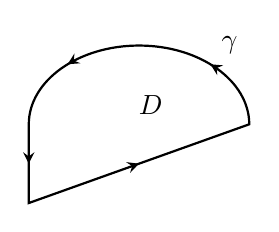
\begin{tikzpicture}
		\path [draw=black,thick,postaction={on each segment={mid arrow=black}}]
		(.2,0) -- (3,1) arc (0:180:1.4 and 1) -- cycle;
		\draw (2.75,2) node {$\gamma$};
		\draw (1.75,1.25) node{$D$};
		\end{tikzpicture}	
	\end{center}
	First, notice that because the curve is simple and closed there are no holes in the region $ D $. Also notice that a direction has been put on the curve. We will use the convention here that the curve $ \gamma $ has a \textit{positive orientation} if it is traced out in a counter-clockwise direction. Another way to think of a positive orientation (that will cover much more general curves as well see later) is that as we traverse the path following the positive orientation the region $ D $ must always be on the left.\\ \\
	Given curves/regions such as this we have the following theorem.
	\begin{theorem}[Green's Theorem]
		Let $ \gamma $ be a positively oriented, piecewise smooth, simple, closed curve and let $ D $ be the region enclosed by the curve. If $ P(x,y) $ and $ Q(x,y) $ have continuous first order partial derivatives on $ D $ then,
		\[ \int\limits_{\gamma} P(x,y)\,dx + Q(x,y)\,dy = \iint\limits_D \left( \frac{\partial Q}{\partial x} - \frac{\partial P}{\partial y} \right)\,dA \]
	\end{theorem}
	\noindent When working with a line integral in which the path satisfies the condition of Green's Theorem we will often denote the line integral as,
	\[ \oint\limits_{\gamma} P(x,y)\,dx + Q(x,y)\,dy \]
	So, Green's theorem will not work on regions that have holes in them. However, many regions do have holes in them. So, let's see how we can deal with those kinds of regions.\\ \\
	Let's start with the following region. Even though this region doesn't have any holes in it the arguments that we're going to go through will be similar to those that we'd need for regions with holes in them, except it will be a little easier to deal with and write down.
	\begin{center}
		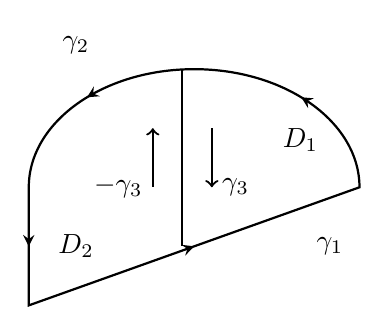
\begin{tikzpicture}[scale=1.5]
		\path [draw=black,thick,postaction={on each segment={mid arrow=black}}]
		(.2,0) -- (3,1) arc (0:180:1.4 and 1) -- cycle;
		\draw[thick] (1.5,2) -- (1.5,0.5);
		\draw[thick,<-] (1.25,1.5) -- (1.25,1) node[left] {$-\gamma_3$};
		\draw[thick,->] (1.75,1.5) -- (1.75,1) node[right] {$\gamma_3$};
		\node at (0.6,.5) {$D_2$};
		\node at (2.5,1.4) {$D_1$};
		\node at (2.75,0.5) {$\gamma_1$};
		\node at (0.6,2.2) {$\gamma_2$};
		\end{tikzpicture}	
	\end{center}
	The region $ D $ will be $ D_1 \cup D_2 $. The boundary of $ D_1 $ is $ \gamma_1 \cup \gamma_3 $ while the boundary of $ D_2 $ is $ \gamma_2 \cup (-\gamma_3) $ and notice that both of these boundaries are positively oriented. As we traverse each boundary the corresponding region is always on the left. Finally, also note that we can think of the whole boundary, $ \gamma $, as,
	\[ \gamma = (\gamma_1 \cup \gamma_3) \cup (\gamma_2 \cup (-\gamma_3)) = \gamma_1 \cup \gamma_2 \]
	Now, let's start with the following double integral and use a basic property of double integrals to break it up.
	\[ \iint\limits_D \left( \frac{\partial Q}{\partial x} - \frac{\partial P}{\partial y} \right)\,dA = \iint\limits_{D_1 \cup D_2} \left( \frac{\partial Q}{\partial x} - \frac{\partial P}{\partial y} \right)\,dA = \iint\limits_{D_1} \left( \frac{\partial Q}{\partial x} - \frac{\partial P}{\partial y} \right)\,dA + \iint\limits_{D_2} \left( \frac{\partial Q}{\partial x} - \frac{\partial P}{\partial y} \right)\,dA \]
	Next, use Green's theorem on each of these and again use the fact that we can break up line integrals into separate line integrals for each portion of the boundary.
	\begin{align*}
		\iint\limits_D \left( \frac{\partial Q}{\partial x} - \frac{\partial P}{\partial y} \right) dA &= \iint\limits_{D_1} \left( \frac{\partial Q}{\partial x} - \frac{\partial P}{\partial y} \right)\,dA + \iint\limits_{D_2} \left( \frac{\partial Q}{\partial x} - \frac{\partial P}{\partial y} \right) dA\\
		&= \oint\limits_{\gamma_1 \cup \gamma_2} P\,dx + Q\,dy + \oint\limits_{\gamma_2 \cup (-\gamma_3)} P\,dx + Q\,dy\\
		&= \oint\limits_{\gamma_1} P\,dx + Q\,dy + \oint\limits_{\gamma_3} P\,dx + Q\,dy + \oint\limits_{\gamma_2} P\,dx + Q\,dy + \oint\limits_{-\gamma_3} P\,dx + Q\,dy    
	\end{align*}
	Recall that changing the orientation of a curve with line integrals with respect to $ x $ and/or $ y $ will simply change the sign on the integral. Using this fact we get,
	\begin{align*}
		\iint\limits_D \left( \frac{\partial Q}{\partial x} - \frac{\partial P}{\partial y} \right)dA &=  \oint\limits_{\gamma_1} P\,dx + Q\,dy + \oint\limits_{\gamma_3} P\,dx + Q\,dy + \oint\limits_{\gamma_2} P\,dx + Q\,dy - \oint\limits_{\gamma_3} P\,dx + Q\,dy\\
		&= 	\oint\limits_{\gamma_1} P\,dx + Q\,dy + \oint\limits_{\gamma_2} P\,dx + Q\,dy\\
		&= \oint\limits_{\gamma_1 \cup \gamma_2} P\,dx + Q\,dy\\
		&= \oint\limits_{\gamma} P\,dx + Q\,dy
	\end{align*}
	So, what did we learn from this? If you think about it this was just a lot of work and all we got out of it was the result from Green's Theorem which we already knew to be true. What this exercise has shown us is that if we break a region up as we did above then the portion of the line integral on the pieces of the curve that are in the middle of the region (each of which are in the opposite direction) will cancel out. This idea will help us in dealing with regions that have holes in them. \\ \\
	We will close out this section with an interesting application of Green's Theorem. Recall that we can determine the area of a region $ D $ with the following double integral.
	\[ A = \iint\limits_D dA \]
	Let's think of this double integral as the result of using Green's Theorem.  In other words, let's assume that
	\[ \frac{\partial Q}{\partial x} - \frac{\partial P}{\partial y} = 1 \]
	and see if we can get some functions $ P $ and $ Q $ that will satisfy this. There are many functions that will satisfy this. Here are some of the more common functions.
	\begin{center}
		\begin{tabular}{c|c|c}
			$ P = 0 $ & $ P = -y $ & $ \displaystyle{P = -\frac{y}{2}} $ \\[8pt]
			$ Q = x $ & $ Q = 0 $ & $ \displaystyle{Q = \frac{x}{2}} $
		\end{tabular}
	\end{center}
	Then, if we use Green's Theorem in reverse we see that the area of the region $ D $ can also be computed by evaluating any of the following line integrals.
	\[ A = \oint\limits_{\gamma} x\,dy = -\oint\limits_{\gamma} y\,dx = \frac{1}{2} \oint\limits_{\gamma} x\,dy - y\,dx \]
	where $ \gamma $ is the boundary of the region $ D $.
	
	\section{Curl and Divergence}
	
	In this section we will introducing new vector operations, the curl and the divergence of a vector.\\ \\
	Given the vector field $ \vec{F} = P(x,y,z)\, \uvec{\i} + Q(x,y,z)\,\uvec{\j} + R(x,y,z)\,\uvec{k} $ the curl of $ \vec{F} $ is defined to be,
	\[ \text{curl }  \vec{F} = (R_y - Q_z)\, \uvec{\i} + (P_z - R_x)\,\uvec{\j} + (Q_x - P_y)\, \uvec{k} \]
	There is actually an easier definition of the curl of a vector field. To use it we will first need to define the $ \nabla $ operator. This is defined to be,
	\[ \nabla = \frac{\partial}{\partial x} \uvec{\i} + \frac{\partial}{\partial y} \uvec{\j} + \frac{\partial}{\partial z} \uvec{k} \]
	Using the $ \nabla $ we can define the curl as the following cross product,
	\[ 
		\text{curl } \vec{F} = \nabla \times \vec{F} = 
			\left|
				\begin{array}{ccc}
					\uvec{\i} & \uvec{\j} & \uvec{k}\\[6pt]
					\dfrac{\partial}{\partial x} & \dfrac{\partial}{\partial y} & \dfrac{\partial}{\partial z}\\[8pt]
					P & Q & R
				\end{array}
			\right| 
	\]
	We have a couple of nice facts that use the curl of a vector field.\\ \\
	\textbf{Facts}
	\begin{enumerate}
		\item If $ f(x,y,z) $ has continuous second order partial derivatives then curl$ (\nabla f) = \vec{0} $.
		\item  If $ \vec{F} $ is a conservative vector field then curl $ \vec{F} = \vec{0} $. This is a direct result of what it means to be a conservative vector field and the previous fact.
		\item If $ \vec{F} $ is defined on all of $ \R^3 $ whose components have continuous first order partial derivative and curl $ \vec{F} = \vec{0} $ then $ \vec{F} $ is a conservative vector field.
	\end{enumerate}
	Next we should talk about a physical interpretation of the curl. Suppose that $ \vec{F} $ is the velocity field of a flowing fluid. Then curl $ \vec{F} $ represents the tendency of particles at the point $ (x,y,z) $ to rotate about the axis that points in the direction of $ \vec{F} $. If curl $ \vec{F} = \vec{0} $ then the fluid is called irrotational.\\ \\
	Given the vector field $ \vec{F} = P(x,y,z)\, \uvec{\i} + Q(x,y,z)\,\uvec{\j} + R(x,y,z)\,\uvec{k} $ the divergence of $ \vec{F} $ is defined to be, 
	\[ \text{div } \vec{F} = \frac{\partial P}{\partial x} + \frac{\partial Q}{\partial y} + \frac{\partial R}{\partial z}  \]
	There is also a definition of the divergence in terms of the $ \nabla $ operator. The divergence can be defined in terms of the following dot product.
	\[ \text{div } \vec{F} = \nabla \cdot \vec{F} \]
	We also have the following fact about the relationship between the curl and the divergence.
	\[ \text{div} (\text{curl } \vec{F}) = 0 \]
	Note that the result is a scalar.\\ \\
	We also have a physical interpretation of the divergence. If we again think of $ \vec{F} $ as the velocity field of a flowing fluid then $ \text{div } \vec{F} $ represents the net rate of change of the mass of the fluid flowing from the point $ (x,y,z) $ per unit volume. This can also be thought of as the tendency of a fluid to diverge from a point. If $ \text{div } \vec{F} = 0 $ then the $ \vec{F} $ is called incompressible.\\ \\
	The final topic in this section is to give two vector forms of Green's Theorem. The first form uses the curl of the vector field and is,
	\[ \oint\limits_{\gamma} \vec{F} \cdot d\vec{r} = \iint\limits_D (\text{curl } \vec{F}) \cdot \uvec{k} \,  dA \]
	The second form uses the divergence. In this case we also need the outward unit normal to the curve $ \gamma $. If the curve is parameterized by 
	\[ \vec{r}(t) = x(t)\,\uvec{\i} + y(t)\,\uvec{\j} \]
	then the outward unit normal is given by,
	\[ \vec{n} = \frac{y'(t)}{||\vec{r}'(t)||} \uvec{\i} - \frac{x'(t)}{||\vec{r}'(t)||} \uvec{\j} \]
	So the vector form of Green's Theorem that uses the divergence is given by,
	\[ \oint\limits_{\gamma} \vec{F} \cdot \vec{n}\,ds = \iint\limits_D \text{div } \vec{F}\,dA \]
	
	\chapter{Surface Integrals}
	
	In the previous chapter we looked at evaluating integrals of functions or vector fields where the points came from a curve in two or three-dimensional space. We now want to extend this idea and integrate functions and vector fields where the points come from a surface in three-dimensional space. These integrals are called surface integrals.
	
	\section{Parametric Surfaces}
	
	Before we get into surface integrals we first need to talk about how to parameterize a surface. When we parameterized a curve we took values of $ t $ from some interval $ [a,b] $ and plugged them into
	\[ \vec{r}(t) = x(t)\,\uvec{\i} + y(t)\,\uvec{\j} + z(t)\,\uvec{k} \]
	and the resulting set of vectors would be the position vectors for the points on the curve. \\ \\
	With surfaces we'll do something similar. We will take points, $ (u,v) $, out of some two-dimensional space $ D $ and plug them into
	\[ \vec{r}(u,v) = x(u,v)\,\uvec{\i} + y(u,v)\,\uvec{\j} + z(u,v)\,\uvec{k} \]
	and the resulting set of vectors will be the position vectors for the points on the surface $ S $ that we are trying to parameterize. This is often called the \textit{parametric representation} of the \textit{parametric surface} $ S $. \\ \\
	Let's take a quick look at a couple of applications. Let's look at finding the tangent plane to the parametric surface $ S $ given by,
	\[ \vec{r}(u,v) = x(u,v)\,\uvec{\i} + y(u,v)\,\uvec{\j} + z(u,v)\,\uvec{k} \]
	First, define
	\begin{align*}
		& \vec{r}_u (u,v) = \frac{\partial x}{\partial u} (u,v) \, \uvec{\i} + \frac{\partial y}{\partial u} (u,v) \, \uvec{\j} + \frac{\partial z}{\partial u} (u,v) \, \uvec{k} \\
		& \vec{r}_v (u,v) = \frac{\partial x}{\partial v} (u,v) \, \uvec{\i} + \frac{\partial y}{\partial v} (u,v) \, \uvec{\j} + \frac{\partial z}{\partial v} (u,v) \, \uvec{k}
	\end{align*}
	Now, provided $ \vec{r}_u \times \vec{r}_v \neq \vec{0} $ it can be shown that the vector $ \vec{r}_u \times \vec{r}_v $ will be orthogonal to the surface $ S $. This means that it can be used for the normal vector that we need in order to write down the equation of a tangent plane. This is an important idea that will be used many times throughout the next couple of sections.\\ \\
	The second application that we want to take a quick look at is the surface area of the parametric surface $ S $ given by,
	\[ \vec{r}(u,v) = x(u,v)\,\uvec{\i} + y(u,v)\,\uvec{\j} + z(u,v)\,\uvec{k} \]
	Provided $ S $ is traced out exactly once as $ (u,v) $ ranges over the points in $ D $ the surface area of $ S $ is given by,
	\[ A = \iint\limits_D ||\vec{r}_u \times \vec{r}_v|| \,dA \]
	
	\section{Surface Integrals}
	
	It is now time to think about integrating functions over some surface, $ S $, in three-dimensional space. Let's start off with a sketch of the surface $ S $ since the notation can get a little confusing once we get into it. Here is a sketch of some surface $ S $.
	\begin{center}
		\tdplotsetmaincoords{70}{120}
		\begin{tikzpicture}[tdplot_main_coords]
		
		% Axis
		\draw[->] (0,0,0) -- (4,0,0) node[left] {$x$};
		\draw[->] (0,0,0) -- (0,4,0) node[right] {$y$};
		\draw[->] (0,0,0) -- (0,0,3) node[above] {$z$};
		
		% Rectangle
		\draw[dashed] (1,0,0) -- (1,1,0);
		\draw[dashed] (2.5,0,0) -- (2.5,1,0);
		\draw[dashed] (0,1,0) -- (1,1,0);
		\draw[dashed] (0,2.5,0) -- (1,2.5,0);
		\draw (1,1,0) -- (2.5,1,0) -- (2.5,2.5,0) -- (1,2.5,0) -- (1,2.5,0) -- (1,1,0);
		\fill[cyan!50,opacity=0.6] (1,1,0) -- (2.5,1,0) -- (2.5,2.5,0) -- (1,2.5,0) -- (1,2.5,0) -- (1,1,0);
		
		% Nodes
		\draw (1,0,0) node[left=1mm] {$a$};
		\draw (2.5,0,0) node[left=1mm] {$b$};
		\draw (0,1,0) node[above] {$c$};
		\draw (0,2.5,0) node[above=] {$d$};
		\draw (2.5,2.5,0) node[below=1mm] {$D$};
		\draw (2,2,2.5) node[above] {$S$};
		
		% Lines to Surface
		\draw[dashed] (1,1,0) -- (1,1,2);
		\draw[dashed] (2.5,1,0) -- (2.5,1,1.5);
		\draw[dashed] (2.5,2.5,0) -- (2.5,2.5,2);
		\draw[dashed] (1,2.5,0) -- (1,2.5,2.5);
		\draw (1,1,2) to[bend left] (2.5,1,1.5);
		\draw (2.5,1,1.5) to[bend right] (2.5,2.5,2);
		\draw (2.5,2.5,2) to[bend right] (1,2.5,2.5);
		\draw (1,2.5,2.5) to[bend left] (1,1,2); 
		\fill[orange!50,opacity=0.6] (1,1,2) to[bend left] (2.5,1,1.5) -- (2.5,1,1.5) to[bend right] (2.5,2.5,2) -- (2.5,2.5,2) to[bend right] (1,2.5,2.5) -- (1,2.5,2.5) to[bend left] (1,1,2);
		\end{tikzpicture}
	\end{center}
	The region $ S $ will lie above (in this case) some region $ D $ that lies in the $ xy $-plane. We used a rectangle here, but it doesn't have to be of course. Also note that we could just as easily looked at a surface $ S $ that was in front of some region $ D $ in the $ yz $-plane or the $ xz $-plane. Do not get so locked into the $ xy $-plane that you can't do problems that have regions in the other two planes. \\ \\
	Now, how we evaluate the surface integral will depend upon how the surface is given to us. There are essentially two separate methods here, although as we will see they are really the same. \\ \\
	First, let's look at the surface integral in which the surface $ S $ is given by $ z = g(x,y) $. In this case the surface integral is,
	\[ \iint\limits_{S} f(x,y,z)\,dS = \iint\limits_D f(x,y,g(x,y)) \sqrt{\left( \frac{\partial g}{\partial x} \right)^2 + \left( \frac{\partial g}{\partial y} \right)^2 + 1}\,dA \]
	Now, we need to be careful here as both of these look like standard double integrals. In fact the integral on the right is a standard double integral. The integral on the left however is a surface integral. The way to tell them apart is by looking at the differentials. The surface integral will have a $ dS $ while the standard double integral will have a $ dA $. \\ \\
	The second method for evaluating a surface integral is for those surfaces that are given by the parameterization,
	\[ \vec{r}(u,v) = x(u,v)\,\uvec{\i} + y(u,v)\,\uvec{\j} + z(u,v)\,\uvec{k} \]
	In these cases the surface integral is,
	\[ \iint\limits_{S} f(x,y,z)\,dS = \iint\limits_D f(\vec{r}(u,v)) || \vec{r}_u \times \vec{r}_v ||\,dA \]
	where $ D $ is the range of the parameters that trace out the surface $ S $.
	
	\section{Surface Integrals of Vector Fields}
	
	Just as we did with line integrals we now need to move on to surface integrals of vector fields. Recall that in line integrals the orientation of the curve we were integrating along could change the answer. The same thing will hold true with surface integrals. So, before we really get into doing surface integrals of vector fields we first need to introduce the idea of an \textit{oriented surface}.\\ \\
	Let's start off with a surface that has two sides that has a tangent plane at every point (except possibly along the boundary). Making this assumption means that every point will have two unit normal vectors, $ \vec{n}_1 $ and $ \vec{n}_2 = -\vec{n}_1 $. This means that every surface will have two sets of normal vectors. The set that we choose will give the surface an orientation. \\ \\
	There is one convention that we will make in regards to certain kinds of oriented surfaces. First we need to define a \textit{closed surface}. A surface $ S $ is closed if it is the boundary of some solid region $ E $. A good example of a closed surface is the surface of a sphere. We say that the closed surface $ S $ has a \textit{positive} orientation if we choose the set of unit normal vectors that point outward from the region $ E $ while the negative orientation will be the set of unit normal vectors that point in towards the region $ E $.\\ \\
	In order to work with surface integrals of vector fields we will need to be able to write down a formula for the unit normal vector corresponding to the orientation that we've chosen to work with.  We have two ways of doing this depending on how the surface has been given to us. First, let's suppose that the function is given by $ z = g(x,y) $. In this case we first define a new function,
	\[ f(x,y,z) = z - g(x,y) \]
	In terms of our new function the surface is then given by the equation $ f(x,y,z) = 0 $.  Now, recall that $ \nabla f $ will be orthogonal (or normal) to the surface given by $ f(x,y,z) = 0 $. This means that we have a normal vector to the surface. The only potential problem is that it might not be a unit normal vector. That isn't a problem since we also know that we can turn any vector into a unit vector by dividing the vector by its length. In our case this is,
	\[ \vec{n} = \frac{\nabla f}{|| \nabla f ||} \]
	In this case it will be convenient to actually compute the gradient vector and plug this into the formula for the normal vector.  Doing this gives,
	\[ \vec{n} = \frac{\nabla f}{|| \nabla f ||} = \frac{-g_x\,\uvec{\i} -g_y\,\uvec{\j} + g_z\,\uvec{k}}{\sqrt{(g_x)^2+(g_y)^2+1}} \]
	Notice that the component of the normal vector in the $ z $-direction is always positive and so this normal vector will generally point upwards. It may not point directly up, but it will have an upwards component to it.\\ \\
	This will be important when we are working with a closed surface and we want the positive orientation. If we know that we can then look at the normal vector and determine if the “positive” orientation should point upwards or downwards. Remember that the ``positive'' orientation must point out of the region and this may mean downwards in places. Of course if it turns out that we need the downward orientation we can always take the negative of this unit vector and we'll get the one that we need. Again, remember that we always have that option when choosing the unit normal vector.\\ \\
	Now, we need to discuss how to find the unit normal vector if the surface is given parametrically as,
	\[ \vec{r}(u,v) = x(u,v)\,\uvec{\i} + y(u,v)\,\uvec{\j} + z(u,v)\,\uvec{k} \]
	In this case recall that the vector $ \vec{r}_u \times \vec{r}_v $ will be normal to the tangent plane at a particular point. But if the vector is normal to the tangent plane at a point then it will also be normal to the surface at that point. So, this is a normal vector. In order to guarantee that it is a unit normal vector we will also need to divide it by its magnitude. So, in the case of parametric surfaces one of the unit normal vectors will be, 
	\[ \vec{n} = \frac{\vec{r}_u \times \vec{r}}{|| \vec{r}_u \times \vec{r}_v ||} \]
	So, given a vector field $ \vec{F} $ with unit normal vector $ \vec{n} $ then the surface integral of $ \vec{F} $ over the surface $ S $ is given by,
	\[ \iint\limits_S \vec{F} \cdot d\vec{S} = \iint\limits_S \vec{F} \cdot \vec{n} \,dS \]
	where the right hand integral is a standard surface integral. This is sometimes called \textit{the flux of} $ \vec{F} $ \textit{across} $ S $.\\ \\
	We will leave this section with a quick interpretation of a surface integral over a vector field. If $ \vec{v} $ is the velocity field of a fluid then the surface integral
	\[ \iint\limits_S \vec{v} \cdot d\vec{S} \]
	represents the volume of fluid flowing through $ S $ per unit time.
	
	\section{Stokes' Theorem}
	
	In this section we are going to take a look at a theorem that is a higher dimensional version of Green's Theorem. In Green's Theorem we related a line integral to a double integral over some region. In this section we are going to relate a line integral to a surface integral. However, before we give the theorem we first need to define the curve that we're going to use in the line integral. Let's start off with the following surface with the indicated orientation.
	\begin{center}
		\tdplotsetmaincoords{60}{110}
		
		%define polar coordinates for some vector
		%TODO: look into using 3d spherical coordinate system
		\pgfmathsetmacro{\radius}{1}
		\pgfmathsetmacro{\thetavec}{0}
		\pgfmathsetmacro{\phivec}{0}
		
		
		\begin{tikzpicture}[scale=2.5,tdplot_main_coords]
			%draw the main coordinate system axes
			\draw[->] (0,0,0) -- (1.5,0,0) node[anchor=south]{$x$};
			\draw[->] (0,0,0) -- (0,1.5,0) node[anchor=north west]{$y$};
			\draw[->] (0,0,0) -- (0,0,1.5) node[anchor=south]{$z$};
			
			\tdplotsetthetaplanecoords{\phivec}
			

			
			\draw[thick,->] (\radius,0,0) arc (0:360:\radius);
			\shade[ball color=blue!10!white,opacity=0.5] (1cm,0) arc (0:-180:1cm and 5mm) arc (180:0:1cm and 1cm);
			
			\draw[thick,->] (1.5,1.5,1.5) -- (1.5,1.75,1.75) node[right] {$\vec{n}$};
			
			\draw (1.2,0.1) node {$\gamma$};
			\draw (0,0.5,1.25) node {$S$};
		\end{tikzpicture}
	\end{center}
	Around the edge of this surface we have a curve $ \gamma $. This curve is called the boundary curve.  The orientation of the surface $ S $ will induce the positive orientation of $ \gamma $. To get the positive orientation of $ \gamma $ think of yourself as walking along the curve. While you are walking along the curve if your head is pointing in the same direction as the unit normal vectors while the surface is on the left then you are walking in the positive direction on $ \gamma $. Now that we have this curve definition out of the way we can give Stokes' Theorem.
	\begin{theorem}[Stokes' Theorem]
		Let $ S $ be an oriented smooth surface that is bounded by a simple, closed, smooth boundary curve $ \gamma $ with positive orientation. Also let $ \vec{F} $ be a vector field then,
		\[ \int\limits_{\gamma} \vec{F} \cdot d\vec{r} = \iint\limits_S \text{curl } \vec{F} \cdot d\vec{S} \]
	\end{theorem}
	\noindent In this theorem note that the surface $ S $ can actually be any surface so long as its boundary curve is given by $ \gamma $. This is something that can be used to our advantage to simplify the surface integral on occasion.
	
	\section{Divergence Theorem}
	
	In the last section we relate surface integrals to triple integrals. We do this using the Divergence Theorem
	\begin{theorem}[Divergence Theorem]
		Let $ E $ be a simple solid region and $ S $ is the boundary surface of $ E $ with positive orientation. Let $ \vec{F} $ be a vector field whose components have continuous first order partial derivatives. Then,
		\[ \iint\limits_S \vec{F} \cdot d\vec{S} = \iiint\limits_E \text{div } \vec{F}\,dV \]
	\end{theorem}
	
	
	
	\addcontentsline{toc}{chapter}{}
	\pagestyle{plain}
	
\end{document}